%!TEX root = ../template.tex
%%%%%%%%%%%%%%%%%%%%%%%%%%%%%%%%%%%%%%%%%%%%%%%%%%%%%%%%%%%%%%%%%%%%
%% chapter5.tex
%% NOVA thesis document file
%%
%% Chapter with lots of dummy text
%%%%%%%%%%%%%%%%%%%%%%%%%%%%%%%%%%%%%%%%%%%%%%%%%%%%%%%%%%%%%%%%%%%%
\chapter{Desenvolvimento do Interpretador Musikla}
O desenvolvimento do projeto pode ser dividido de grosso modo em três camadas. Nelas são cobertos um grupo abrangente de aspetos tanto da área do processamento de linguagens e do desenvolvimento de \acrshort{dsl}'s, da teoria musical, e do processamento digital de áudio. 

Na camada da linguagem esteve mais proeminente a área de processamento de linguagens, por motivos óbvios. Mas nas decisões tomadas durante o desenvolvimento desta camada, estiveram sempre presentes também as necessidades específicas que a teoria musical (e a sua notação) impõem numa linguagem de programação.

Do mesmo modo, o interpretador faz claramente uso de tópicos do domínio do processamento de linguagens, mas é ainda mais fortemente influenciado pelas restrições  e requisitos impostos pela componente musical da linguagem. Esta influencia a forma e a semântica da execução dos vários operadores disponibilizados.

A última camada, de desenvolvimento de uma biblioteca, afeta composta pelos objetos e procedimentos que têm como objetivo facilitar a utilização da linguagem. Para isso foi necessário identificar os casos de utilização mais comuns e prioritários, de modo a guiar a construção destas interfaces para refletirem uma utilização real da linguagem e da aplicação.

\section{Análise Sintática}
A camada sintática da aplicação pode ser conceptualmente dividida em duas fases:
\begin{description}
    \item[Sintaxe] Esta fase caracteriza-se por delinear qual a sintaxe usada pela linguagem, bem como os construtores e operadores suportados;
    \item[Parser] Nesta fase foi desenvolvido um \textit{parser} em \textit{Python}, responsável por converter o código fonte da linguagem numa \acrfull{ast};
\end{description}

No entanto, a realidade é que a abordagem seguida (não só nesta camada mas como em todo o projeto) foi mais iterativa, dividindo cada fase em porções semi-independentes e intercalando as várias porções das diversas fases. Esta abordagem tem a vantagem de permitir ir testando e experimentando com o projeto mais cedo do que seria possível com um modelo de desenvolvimento em cascata.

\subsection{Descrição Sintática}
A sintaxe da linguagem é fortemente inspirada nas usualmente chamadas linguagens da família C, com recurso a parênteses curvos e chavetas para delínear os vários blocos da linguagem. No entanto, as expressões são complementadas com um novo conjunto de literais e operadores dedicados à componente músical da linguagem. Conseguir juntar estes dois mundos traz consigo alguns desafios que serão discutidos mais em detalhe em cada umas das secções seguintes.

\subsubsection{\textbf{Constantes ou Literais}}
Literais referem-se ao conceito de sintaxe desenhada com o propósito de descrever dados (literais) no código. São usados em quase todas as linguagens de programação (e na nossa também) para descrever números, \textit{strings} e booleanos.

A maior diferença nesta área entre a nossa linguagem e as restantes, foi a adição de literais responsáveis por modelar conceitos musicais, como notas, pausas e acordes. Esta sintaxe, tal como já foi mencionado anteriormente, foi inspirada pelo projeto \textit{abc notation}, com algumas modificações.

\subsubsection{\textbf{Notas e Pausas}}
A sintaxe de notas descrição de notas é composta por quatro componentes: \textbf{acidentes}, \textbf{\textit{pitch}} (obrigatório), \textbf{oitava} e \textbf{duração}.

\begin{lstlisting}[caption=Expressão Regular que identifica uma nota (quebras de linha adicionadas apenas para claridade de leitura)]
[_^]*
[a-gA-G]
[',]*
([0-9]*\/)?[0-9]*
\end{lstlisting}

O \textit{pitch} refere-se à nota (ou frequência) que deve ser tocada. O \textbf{C médio} (também conhecido como C4) é descrito simplesmente como \texttt{C}. É possível descer uma ou mais oitavas acrescentando uma ou mais vírgulas \texttt{,}. Para subir uma oitava, podemos primeiro substituir as letras maiúsculas por minúsculas. Para subir ainda mais oitavas, podemos acrescentar uma ou mais pelicas \texttt{'}. Para subir ou descer semitons, podemos prefixar as notas com os acidentes \textbf{\texttt{\textasciicircum{}}} e \textbf{\texttt{\_}}, respetivamente.

As pausas são mais simples, sendo compostas simplesmente pela letra \texttt{r} seguida da sua \textbf{duração} (usando as mesma sintaxe das notas).

\subsubsection{\textbf{Acordes}}
Para definir acordes na linguagem, colocam-se várias notas dentro de parênteses retos. A notação usada para cada nota inclui os seus três primeiros componentes (acidentes, \textit{pitch} e oitava), mas exclui a duração. Em vez de definir a duração em cada nota, esta é definida globalmente no acorde após fechar os parênteses retos.

Por conveniência, para evitar ao utilizador ter de introduzir todas as notas de um acorde manualmente, temos uma sintaxe abreviada para os tipos de acordes mais comuns, onde é apenas necessário introduzir a nota base seguido do tipo de acorde. Esta sintaxe irá suportar mais tipos no futuro, sendo atualmente possível usar os seguintes sufixos:

\begin{table}[h]
\centering
\def\arraystretch{1.3}
\begin{tabular}{|l|c|}
\hline
\textbf{}        & \textbf{Abreviaturas}           \\ \hline
\textbf{Tríades} & M, m, aug, dim, +                \\ \hline
\textbf{Quinta}  & 5                                \\ \hline
\textbf{Sétimas} & m7, M7, dom7, 7, m7b5, dim7, mM7 \\ \hline
\end{tabular}
\caption{Lista de abreviaturas possíveis de serem acrescentadas a seguir a uma nota para especificar um acorde.}
\label{tab:modifiers-list}
\end{table}

A decisão de envolver cada acorde com parênteses retos deveu-se ao facto de muitas abreviaturas serem já populares no domínio da notação musical, e como tal o ideal era não as mudar. No entanto, algumas dessas abreviaturas poderiam entrar em conflito com outros componentes da declaração da nota. Por exemplo, \texttt{C7} poderia ser tanto um acorde de sétima como uma nota com duração de 7. Com a separação por parênteses retos, a ambiguidade deixa de existir, sendo óbvio que \texttt{[C7]} é um acorde de sétima, e \texttt{C7} é uma nota com duração 7.

\begin{lstlisting}[caption={Exemplos de três definições de acordes possíveis}] 
[CFG]/4 [^Fm] [C5]2
\end{lstlisting}

\subsubsection{\textbf{Modificadores de Voz}}

Para além de permitir descrever notas, também é possível ter modificadores de voz que permitem alterar certas propriedades das notas e acordes. Duas destas propriedades (duração e oitava) podem ser depois customizadas em cada nota ou acorde, como já vimos. No entanto, em vez de estes valores substituírem simplesmente os valores predefinidos, eles ``complementam-se''.

Ou seja, se declararmos por exemplo que a duração base das notas é $\frac{1}{4}$. Quando definirmos alguma nota a seguir com a duração de $\frac{1}{2}$, a sua duração real irá ser calculada da seguinte forma $\frac{1}{4} \times \frac{1}{2} = \frac{1}{8}$.

Do mesmo modo, quando definimos por exemplo a oitava base como $5$ (o valor predefinido é $4$), a nota \texttt{C,} passa a representar a oitava $5 - 1 = 4$ (por predefinição seria $4 - 1 = 3$) (nota que aqui estamos a falar de oitavas indexadas a zero. No mundo da música elas são geralmente indexadas a um).

Podemos então ver a lista dos modificadores aceites pela linguagem, bem como exemplos de utilização e os seus respetivos valores predefinidos (usados quando nenhum modificador desse tipo é aplicado).

\begin{table}[h]
\centering
\def\arraystretch{1.3}
\begin{tabular}{|l|c|c|c|}
\hline
\textbf{Nome} & \textbf{Modificador}                                            & \textbf{Exemplo}                                        & \textbf{Predefinição} \\ \hline
Instrumento   & I$N$                                                            & I46                                                     & I0           \\ \hline
Velocidade    & V$N$                                                            & V100                                                    & V127         \\ \hline
Tempo         & T$N$                                                            & T120                                                    & T60          \\ \hline
Duração       & \begin{tabular}[c]{@{}c@{}}L$N$\\ L/$N$\\ L$D$/$N$\end{tabular} & \begin{tabular}[c]{@{}c@{}}L2\\ L/4\\ L3/8\end{tabular} & L1           \\ \hline
Oitava        & O$N$                                                            & O2                                                      & O4           \\ \hline
Compasso      & S$D$/$N$                                                        & S3/4                                                    & S4/4         \\ \hline
\end{tabular}
\caption{Lista de modificadores e exemplos da sua utilização}
\label{tab:modifiers-list}
\end{table}

\subsubsection{\textbf{Variáveis e Funções}}
Uma das consequências da introdução da sintaxe de notas literais foi a impossibilidade de ter variáveis com certos nomes. Uma variável chamada \textbf{\texttt{a}}, por exemplo, iria entrar em conflito com a nota do mesmo nome. Do mesmo modo, uma variável chamada \texttt{i1} iria entrar em conflito com o modificador de instrumento. 

Em vez de criar casos de exceção para as variáveis que possam ter nomes que conflitam com outros construtores sintáticos, seguimos o exemplo de outras linguagens como \textit{PHP}, \textit{Perl} ou \textit{Powershell}, e decidimos prefixar as nossas variáveis com o carácter \texttt{\$}.

No caso das funções foi possível evitar a ambiguidade (e do mesmo modo a obrigatoriedade de as prefixar com um carácter) devido ao facto de as funções terem obrigatoriamente um par de parênteses (sem espaço entre os mesmos e o nome da função) quando são chamadas.

No entanto não quer dizer que as funções passaram imunes à introdução das literais de música. Uma vez que a vírgula é usada para mudar a oitava de uma nota (e foi escolhida de forma a manter compatibilidade com a sintaxe do projeto \textit{abc notation}), existem casos em que esta não pode ser utilizada para separar os argumentos passados a uma função.

Por exemplo, dada a expressão \texttt{function\_name(C, A, \$a, 2)}, quantos argumentos podemos concluir que a mesma tem? Quatro? A resposta correta seria dois, pois as duas primeiras vírgulas poderiam pertencer à nota ou ao separador da função. Mas neste caso a nota teria prioridade na nossa gramática, pelo que \texttt{C, A, \$a} seria o primeiro argumento, e \texttt{2} seria o segundo.

A solução tomada inicialmente foi utilizar ponto-e-vírgula para substituir a vírgula como separador de argumentos nas funções. E enquanto isso resolveu os problemas de ambiguidade, tornou-se óbvio à medida que que a linguagem foi avançando, que a prevalência da vírgula como separador de argumentos em quase todas as linguagens de programação mais populares fazia com que houvesse um custo mental de mudança de contexto sempre que alguém mudava de alguma linguagem para a nossa, e vice-versa.

A solução escolhida no final foi um compromisso entre as duas opções: tanto a vírgula como o ponto-e-vírgula podem ser usados como separadores de argumentos, com a exceção de quando o argumento é uma nota musical, onde o ponto-e-vírgula tem de ser obrigatoriamente usado. Assim sendo, poderíamos rescrever o exemplo anterior da seguinte forma \texttt{function\_name(C; A; \$a, 2)}, passando a função a receber agora os quatro argumentos como seria inicialmente esperado.

\subsection{Gramática}
Aqui vamos analisar brevemente uma versão simplificada da gramática (a versão completa usada pela aplicação pode ser vista no Apêndice \ref{grammar}). Nesta versão simplificada, incluída para facilitar a leitura, não aborda detalhes como recursividade à esquerda, ou precedência de operadores. Obviamente, na gramática real foram usadas as técnicas usuais para cobrir esses casos.
A notação da linguagem Musikla cobre várias sub-gramáticas, tanto da parte musícal, descrição de teclados mas também instruções e expressões de uma programação de linguagem genérica, que iremos abordar de seguida.

\subsubsection{Corpo}
Comecemos pela descrição geral do corpo de um ficheiro Musikla. O corpo é composto por uma lista de \textit{statements} (ou instruções) que são obrigatoriamente separados por pontos e vírgula (sendo apenas o último opcional). 

No fim de todas as instruções, opcionalmente, o utilizador também pode inserir um bloco de código \textit{Python} (que é denotado pelo prefixo \texttt{@python} e consome todo o texto até ao fim).

\begin{lstlisting}[caption={Produções base da gramática},language={}]
main <- body python? EOF

body <- statement ( ";" statement )* ";"?

python <- "@python" python_body

python_body <- ( r".*" r"\r?\n"? )*
\end{lstlisting}

Ao longo da gramática são também usadas produções triviais, como inteiros, \textit{strings}, booleanos entre outras. Sendo tão comuns e simples, não vale a pena estar a descrevê-las todas. Deixamos no entanto aqui duas produções que vão ser usadas, mas cujas definições podem ser ligeiramente diferentes do usual.

\begin{lstlisting}[caption={Produções base da gramática},language={}]
sep = r"[,;]"

identifier <- r"[a-zA-Z\_]" r"[a-zA-Z0-9\_\\]"*
\end{lstlisting}

\subsubsection{Instruções}

\begin{lstlisting}[caption={Produções de instruções na gramática},language={}]
statement <- assignment / voice_declaration / import / for / while / if / return / expression

import <- "import" identifier
        / "import" string_value

assignment <- expression assignment_infix? "=" expression

assignment_infix <- "+" / "-" / "/" / "*" / "|" / "&"

voice_declaration <- ":" identifier "=" voice_declaration_body

voice_declaration_body <- ":" identifier "(" expression ")"
                        / expression

for_variables <- variable ( (',' / ';') variable )*

for_loop_head <- "for" "(" for_variables "in" value_expression ".." value_expression ")"
               / "for" "(" for_variables "in" value_expression ")"

for <- for_loop_head "{" body? "}"

while <- "while" "(" expression ")" "{" body "}"

if <- "if" "(" expression ")" "{" body "}" "else" "{" body "}"
    / "if" "(" expression ")" "{" body "}"

return_statement <- "return" expression?
\end{lstlisting}
A nível de instruções, a nossa gramática segue o habitual e não carece de muitos comentários.

\subsubsection{Expressões}
As nossas expressões, como já foi dito, estão aqui listadas. O conceito de recursividade à esquerda é ignorado nestes exemplos por questões de simplicidade, e a precedência de operadores binários é denotada apenas informalmente pela ordem das produções, começando pelo operador com menos precedência e subindo até aos operadores com mais precedência.

Os \textit{arrays} e \textit{objetos} são bastante similares à sintaxe usada no \textit{python}, com a distinção de que para evitar ambiguidades com outras produções da gramática, têm de ser precedidos com o símbolo \texttt{@}.

Alguns das outras regras (como notas ou teclados, que são aceites como expressões) serão descritas nas próximas sub-secções.
\begin{lstlisting}[caption={Produções de expressões na gramática},language={}]
expression <- expression "|" expression
            / expression ("and" / "or") expression
            / expression (">=" / ">" / "==" / "!=" / "<=" / "<") expression
            / expression ("+" / "-") expression
            / expression ("**" / "*" / "/") expression
            / expression expression
            / expression "::" identifier
            / expression "::" "[" expression "]"
            / ( expression / identifier ) "(" parameters ")"
            / "not" expression
            / "(" expression ")"
            / "{" body "}"
            / variable  / function_declaration  / python_expression
            / keyboard / note / chord / rest   / modifier
            / integer / none / bool  / string / array / object

variable <- "$" identifier

parameters <- positional_parameters ( parameters_separator named_parameters )?
            / named_parameter?

positional_parameters <- expression ( r"[,;]" expression )*

named_parameters <- named_parameter ( r"[,;]" named_parameter )*

named_parameter <- identifier '=' expression

function_declaration <- "fun" identifier? "(" argument_list? ")" "{" body "}"
                      / "fun" identifier? "(" argument_list? ")" "=>" expression

argument_list <- argument ( (',' / ';') argument )*

argument <- ("expr" / "ref" / "in")? "$" identifier ("=" expression)?

python_expression <- "@py" "{" python_expression_body "}"

python_expression_body <- r"[^\}]*"

array <- "@[" "]"
        / "@[" expression ( sep expression )* "]"

object <- "@{" "}"
        / "@{" object_item ( sep object_item )* "}"

object_item <- object_key _ '=' _ expression

object_key <- identifier / float / integer / string
\end{lstlisting}

\subsubsection{Música}
No que toca a música, a sintaxe tenta seguir ao máximo a notação usada pelo projeto \textbf{abc}. As suas particularidades também já foram discutidas em bastante detalhe ao longo deste documento, pelo que as produções colocadas aqui não necessitam de muitos comentários.
\begin{lstlisting}[caption={Produções de elementos musicais na gramática},language={}]
note <- note_pitch note_value?

note_value <- "/" integer
            / integer "/" integer
            / integer

note_pitch <- note_accidental note_pitch_octave

note_accidental <- "^" / "^^" / "__" / "_" / ""

note_pitch_octave <- r"[cdefgab]" "'"*
                   / r"[CDEFGAB]" ","*

chord <- "[" note_pitch chord_suffix "]" note_value?
       / "[" note_pitch+ "]" note_value?

chord_suffix <- 'm7' / 'M7' / 'dom7' / '7' / 'm7b5' / 'dim7' / 'mM7'
              / '5'
              / 'M' / 'm' / 'aug' / 'dim' / '+'

rest <- "r" note_value?

modifier
    <- r"[tT]" integer
     / r"[vV]" integer
     / r"[iI]" integer
     / r"[lL]" note_value
     / r"[sS]" integer "/" integer
     / r"[sS]" integer
     / r"[oO]" integer
     / ":" identifier
\end{lstlisting}

\subsubsection{Teclados}
As produções para descrever teclados são um ponto fulcral na gramática e na utilização da linguagem em geral. Quisemos que elas permitissem descrever teclados de uma forma concisa, mas ainda assim dando bastante poder ao utilizador na forma como o utiliza.

Com isso em mente, podemos ver que os teclados têm um corpo que difere do corpo geral da linguagem, mas ao mesmo tempo mantém algumas similaridades, nomeadamente, o facto de cada instrução no corpo ser separada por um ponto e vírgula.

No entanto, as instruções no corpo de um teclado são diferentes: a instrução mais básica, denominada por \textit{shortcut}, pode ser imaginada como um par tecla e ação (com mais alguma informação adicional, como por exemplo, argumentos do evento).

Para além disso, também há outras instruções aceites que permitem aos nossos teclados serem gerados dinamicamente: \texttt{for}, \texttt{while} e \texttt{if}. Os cabeçalhos destas instruções são de grosso modo iguais aos das suas versões \textit{general-purpose}, mas nos seus corpos aceitam só instruções de teclados também.

Por fim, existe mais uma instrução válida, \textit{block}, que permite colocar instruções normais e sem restrições, envoltas num par de chavetas. Isto é útil quando precisamos de declarar alguma variável dentro do teclado para evitar, por exemplo, repetir um pedaço de código múltiplas vezes.

\begin{lstlisting}[caption={Produções associadas a teclados na gramática},language={}]
keyboard <- "@keyboard" identifier* group? "{" keyboard_body "}"

keyboard_body <- keyboard_body_statement ( ";" keyboard_body_statement )* ";"?

keyboard_body_statement <- keyboard_for
                         / keyboard_while
                         / keyboard_if
                         / keyboard_block
                         / keyboard_shortcut

keyboard_for <- for_loop_head "{" keyboard_body "}"

keyboard_while <- "while" "(" expression ")" "{" keyboard_body "}"

keyboard_if <- "if" "(" expression ")" "{" keyboard_body "}" "else" "{" keyboard_body "}"
             / "if" "(" expression ")" "{" keyboard_body "}"

keyboard_block <- "{" body "}"

keyboard_shortcut <- keyboard_shortcut_key keyboard_argument_list? ":" expression

keyboard_shortcut_key <- identifier ("+" identifier)* identifier*
                       / string_value identifier*
                       / "[" expression "]" identifier*

keyboard_argument_list <- "(" ( variable ( r"[,;]" variable )* )? ")"
\end{lstlisting}

% começa cinco linhas numa nova página
\subsection{Reconhecedor Sintático}
Para implementar o reconhecedor sintático ou \textit{parser} da linguagem, foi utilizado o módulo \textit{Python} \textbf{Arpeggio}, um módulo que implementa um algoritmo de \textit{parsing} \acrshort{peg} descendente recursivo com recurso opcional a \textit{memoization} para melhorar a \textit{performance}.

\begin{lstlisting}[caption={Excerto da gramática desenvolvida}]
main <- body EOF;

body <- statement ( ";" statement )* _ ";"? _
    / ""
    ;

// Statements
statement <- _ ( var_declaration / voice_declaration / function_declaration / for_loop_statement / while_loop_statement / if_statement / expression ) _;

var_declaration <- "$" namespaced _ "=" _ expression;
// ...
\end{lstlisting}

A gramática \acrshort{peg} desenvolvida para o projeto foi depois complementada por uma classe \textbf{Parser}, responsável por gerar a \acrshort{ast} da linguagem. Para isso recorremos ao \textit{Visitor Pattern}, com um método para cada regra não-terminal da gramática (todos prefixados com \texttt{visit\_}).

\begin{lstlisting}[caption={Métodos responsáveis por criarem a AST}]
def visit_body ( self, node, children ): ...

def visit_comment ( self, node, children ): ...

def visit_statement ( self, node, children ): ...

def visit_var_declaration ( self, node, children ): ...
\end{lstlisting}

\subsection{Tooling}
Para além da gramática e do \textit{parser} da linguagem, que são indispensáveis para o funcionamento do projeto, foram também implementados algumas funcionalidades adicionais com o intuito de facilitar a utilização da nossa linguagem, que só vamos cobrir brevemente.

\subsubsection{Syntax Highlighting}
Para oferecer \textit{syntax highlighting} para a nossa linguagem, que a nosso ver torna a experiência de programar com a mesma muito mais agradável, utilizamos uma linguagem chamada \textbf{Iro}\footnote{\url{https://eeyo.io/iro/}}. Esta linguagem é uma \acrshort{dsl} que permite descrever a sintaxe através de expressões regulares, e associar estilos a cada uma. 

\begin{lstlisting}[caption={Pequeno excerto da definição da linguagem escrito em Iro}]
:pattern {
    regex          \= (=>|<=|>=|==|!=|[=\*\|\+\-\/]|>=)
    styles []       = .operator;
}

: pattern {
    regex          \= (#.*)
    styles []       = .comment;
}
\end{lstlisting}

A sua grande vantagem é permitir, a partir de uma única definição, gerar versões em formatos específicos suportados por vários editores, como por exemplo o \textit{TextMate}, \textit{Visual Studio Code}, \textit{Atom}, \textit{Sublime 3}, ou até convenientemente para o formato suportado pelo popular módulo \textit{Python} \textbf{Pygments}. Usamos este módulo para colorir os exemplos de código na nossa documentação, como iremos ver na secção seguinte.


\begin{figure}[ht]
  \centering
  {%
  \setlength{\fboxsep}{0pt}%
  \setlength{\fboxrule}{0pt}%
  \fbox{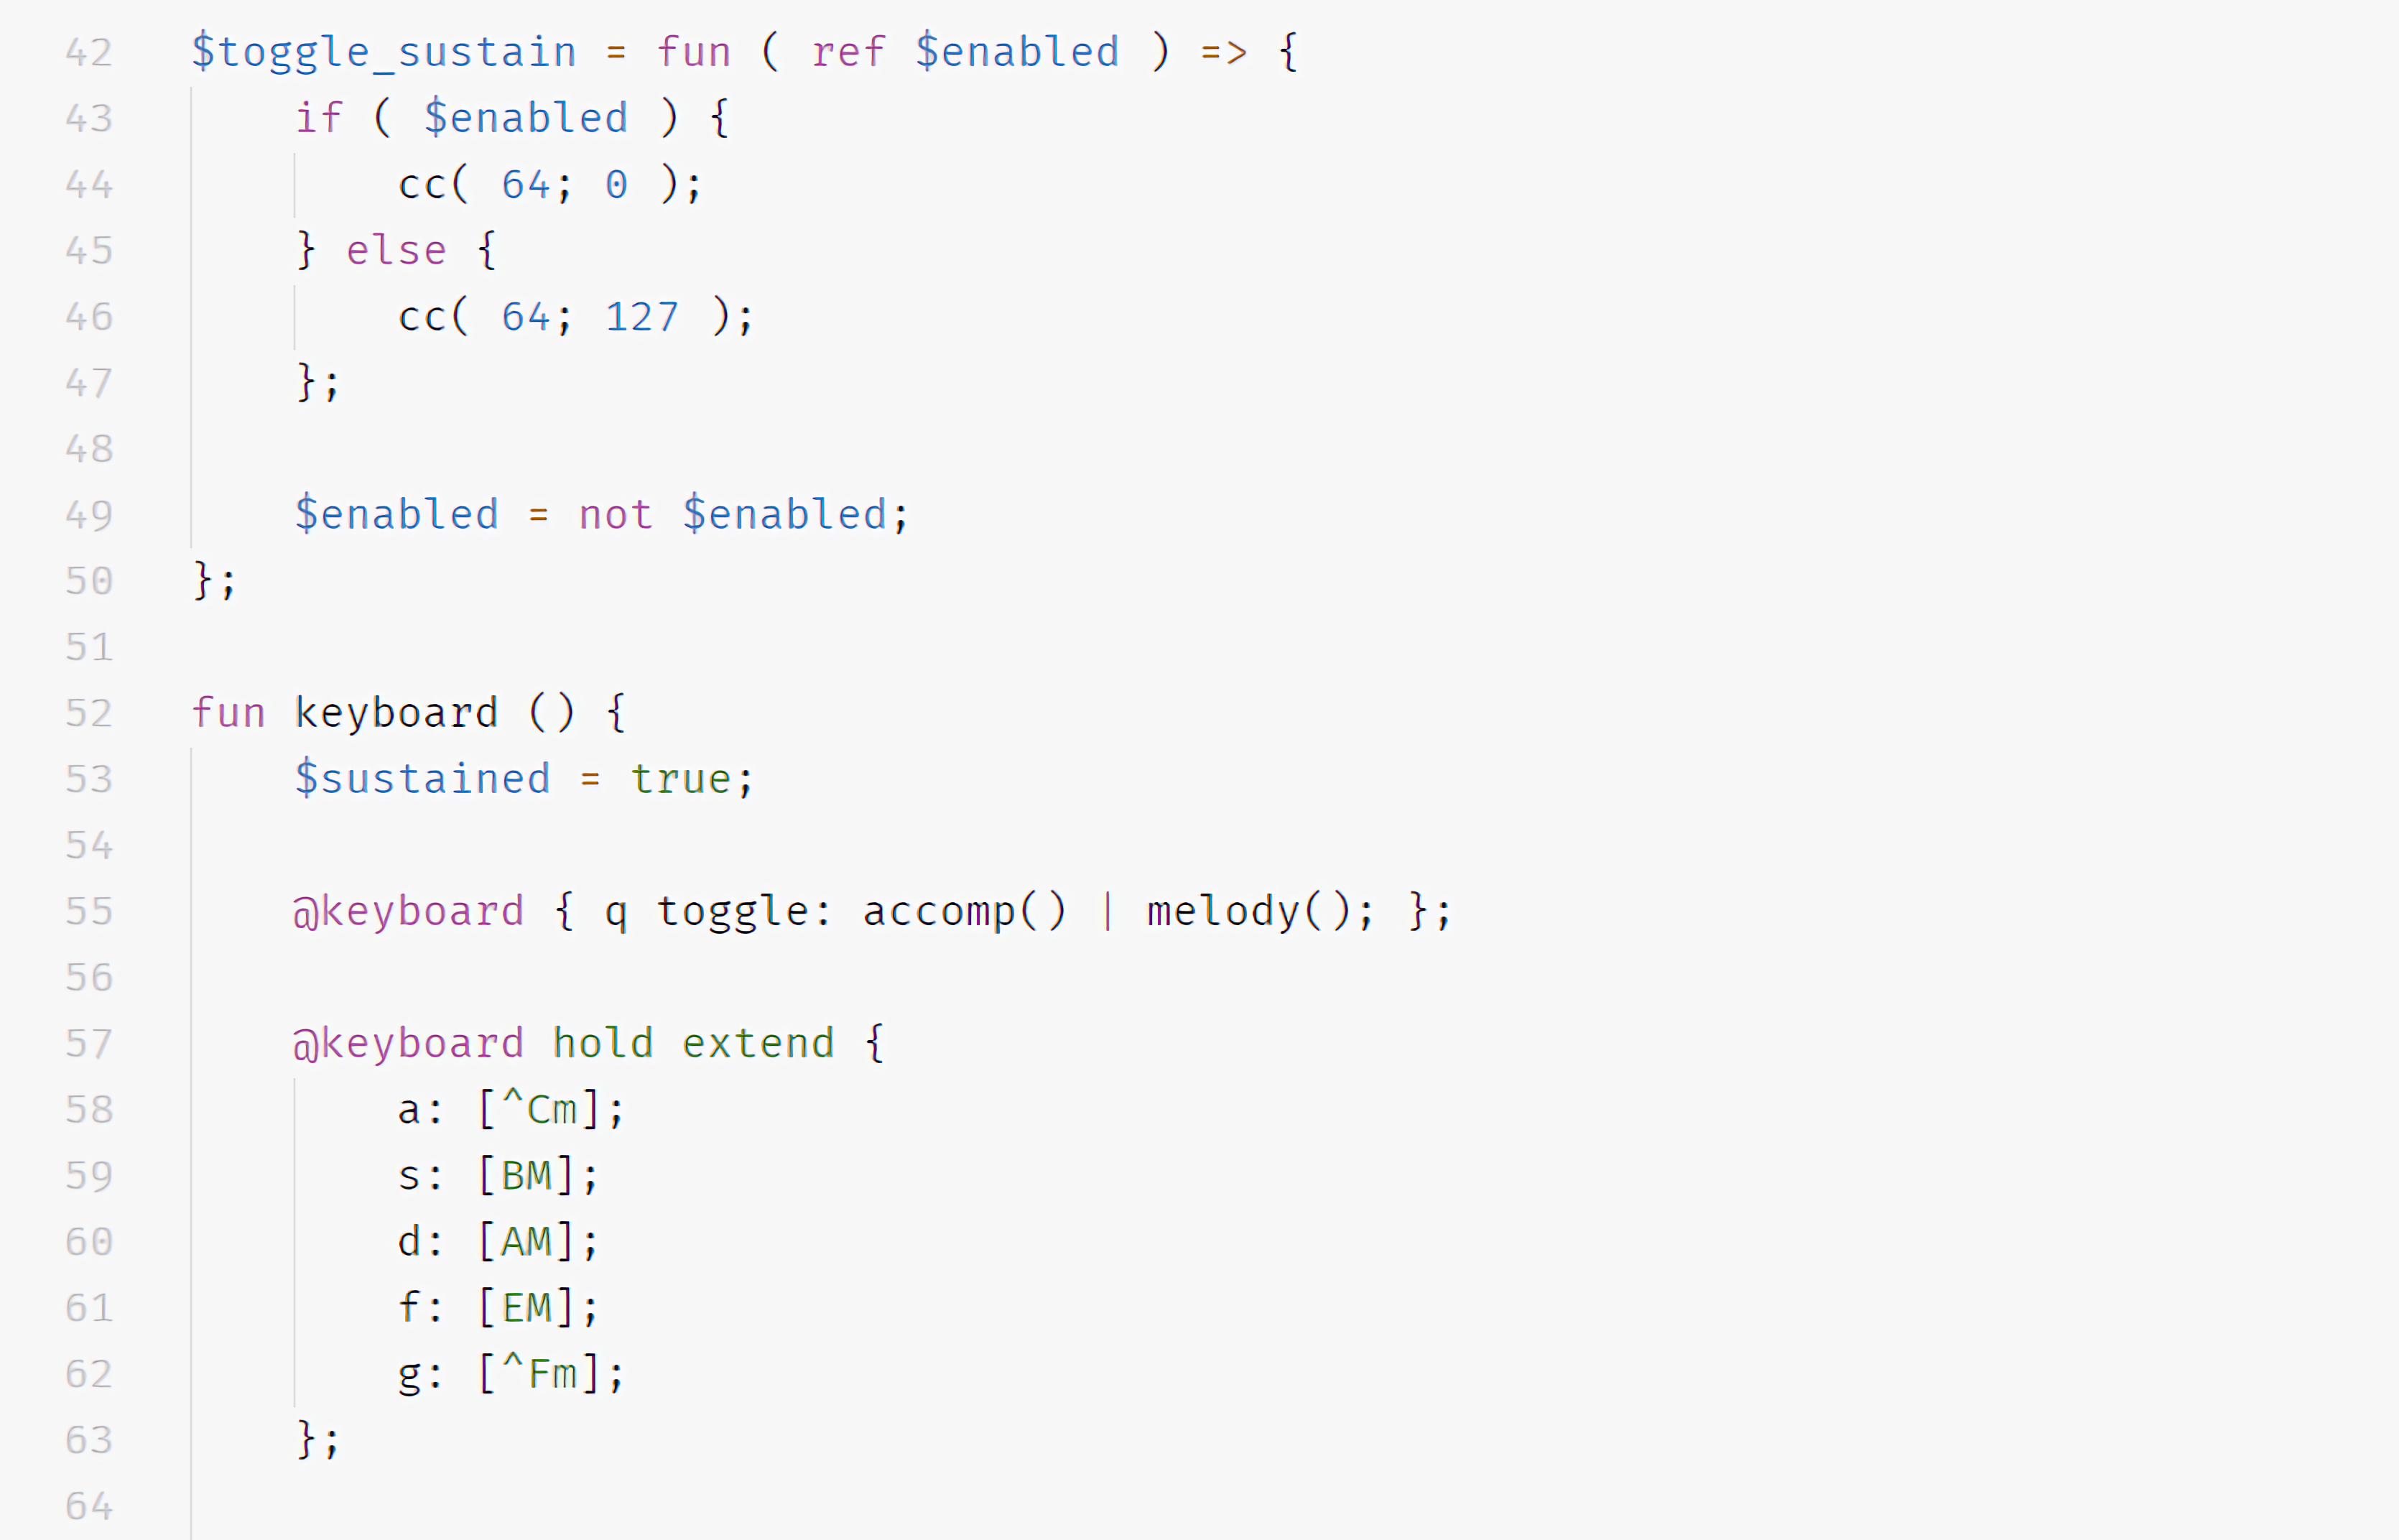
\includegraphics[width=.95\linewidth]{./img/syntax_highlight.png}}%
  }%
  \caption{\textit{Syntax highlighting} da linguagem MusiKLa no editor Visual Studio Code}
  \label{fig:syntax-highlighting-code}
\end{figure}

\newpage

\subsubsection{Documentação}
Também foi escrita documentação para a linguagem disponível \href{https://pedromsilvapt.github.io/miei-dissertation/}{online}\footnote{\url{https://pedromsilvapt.github.io/miei-dissertation/}}, que inclui informação sobre a sintaxe, exemplos de \textit{scripts} funcionais escritos em \textit{musikla}, e uma \acrshort{api} com a descrição das várias funções disponibilizadas, as suas assinaturas e alguns exemplos de utilização.

A documentação foi escrita em \textit{Markdown}, e convertida para \acrshort{html} usando o projeto \textbf{mkdocs}\footnote{\url{https://www.mkdocs.org/}}. Os exemplos de código disponibilizados na documentação são coloridos pelo módulo \textbf{Pygments}, usando a definição de linguagem que descrevemos na secção anterior.

\begin{figure}[ht]
  \centering
  {%
  \setlength{\fboxsep}{0pt}%
  \setlength{\fboxrule}{0pt}%
  \fbox{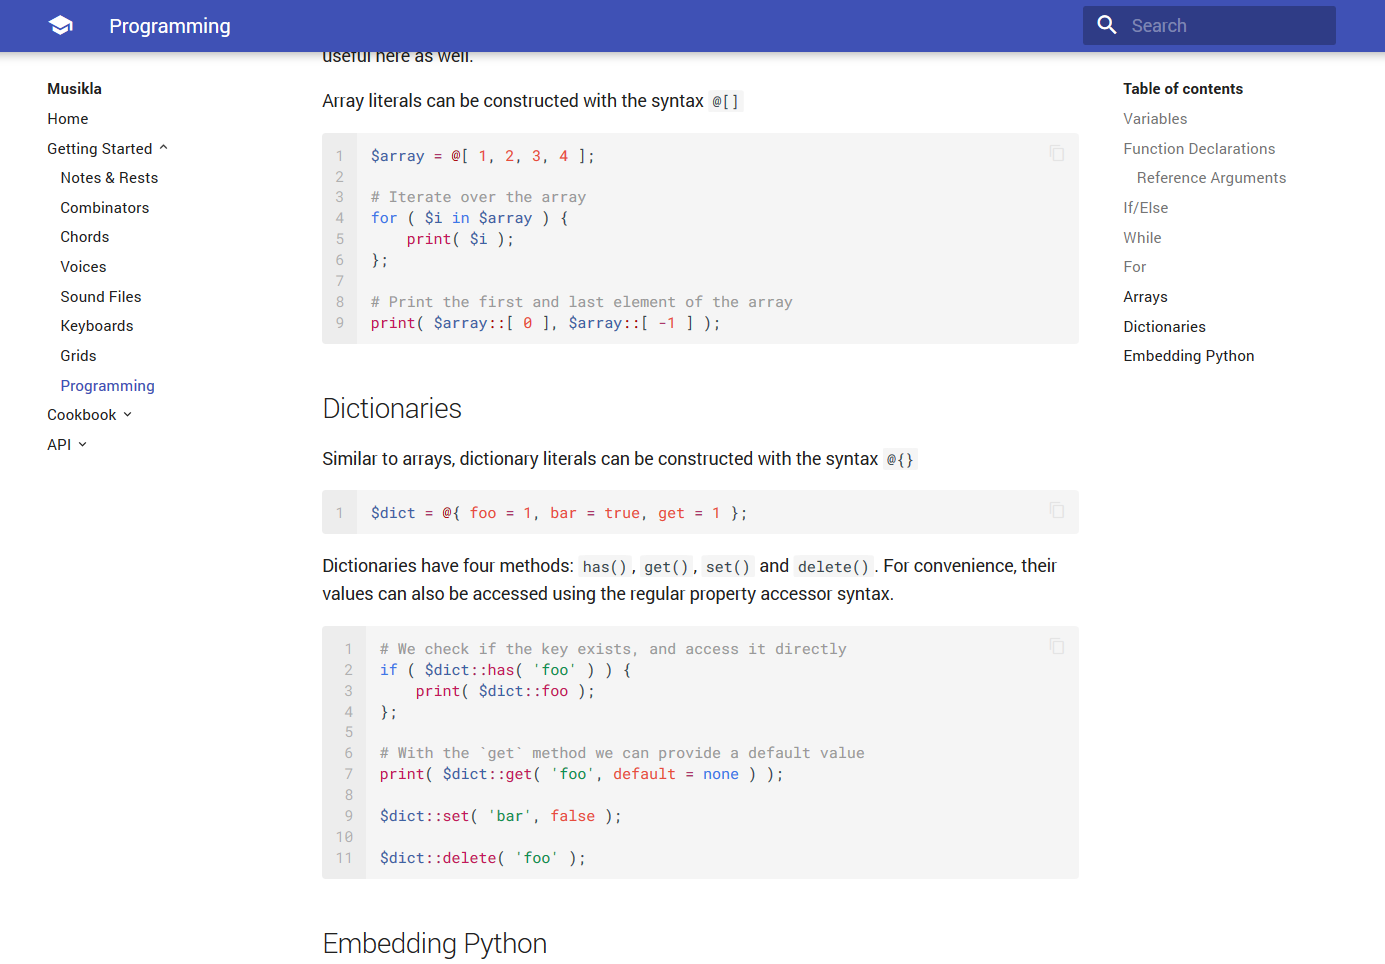
\includegraphics[width=.95\linewidth]{./img/documentation.png}}%
  }%
  \caption{Captura de ecrã da página de documentação da linguagem}
  \label{fig:documentation-screenshot}
\end{figure}

\subsubsection{Relatórios de Erros}
A aplicação de linha de comandos que interpreta a linguagem também dispõe de um componente responsável por, quando ocorre algum erro relacionado com a linguagem, imprimir para o terminal o sítio onde o erro ocorreu, bem como a mensagem a descrever o erro.

Existem dois tipos de erros possíveis: erros de sintaxe, que ocorrem durante a fase de \textit{parse} quando algum carácter está no sítio errado; e erros de execução, que ocorrem quando a linguagem está a executar e podem ter causas variadas.

\begin{figure}[ht]
  \centering
  {%
  \setlength{\fboxsep}{0pt}%
  \setlength{\fboxrule}{0pt}%
  \fbox{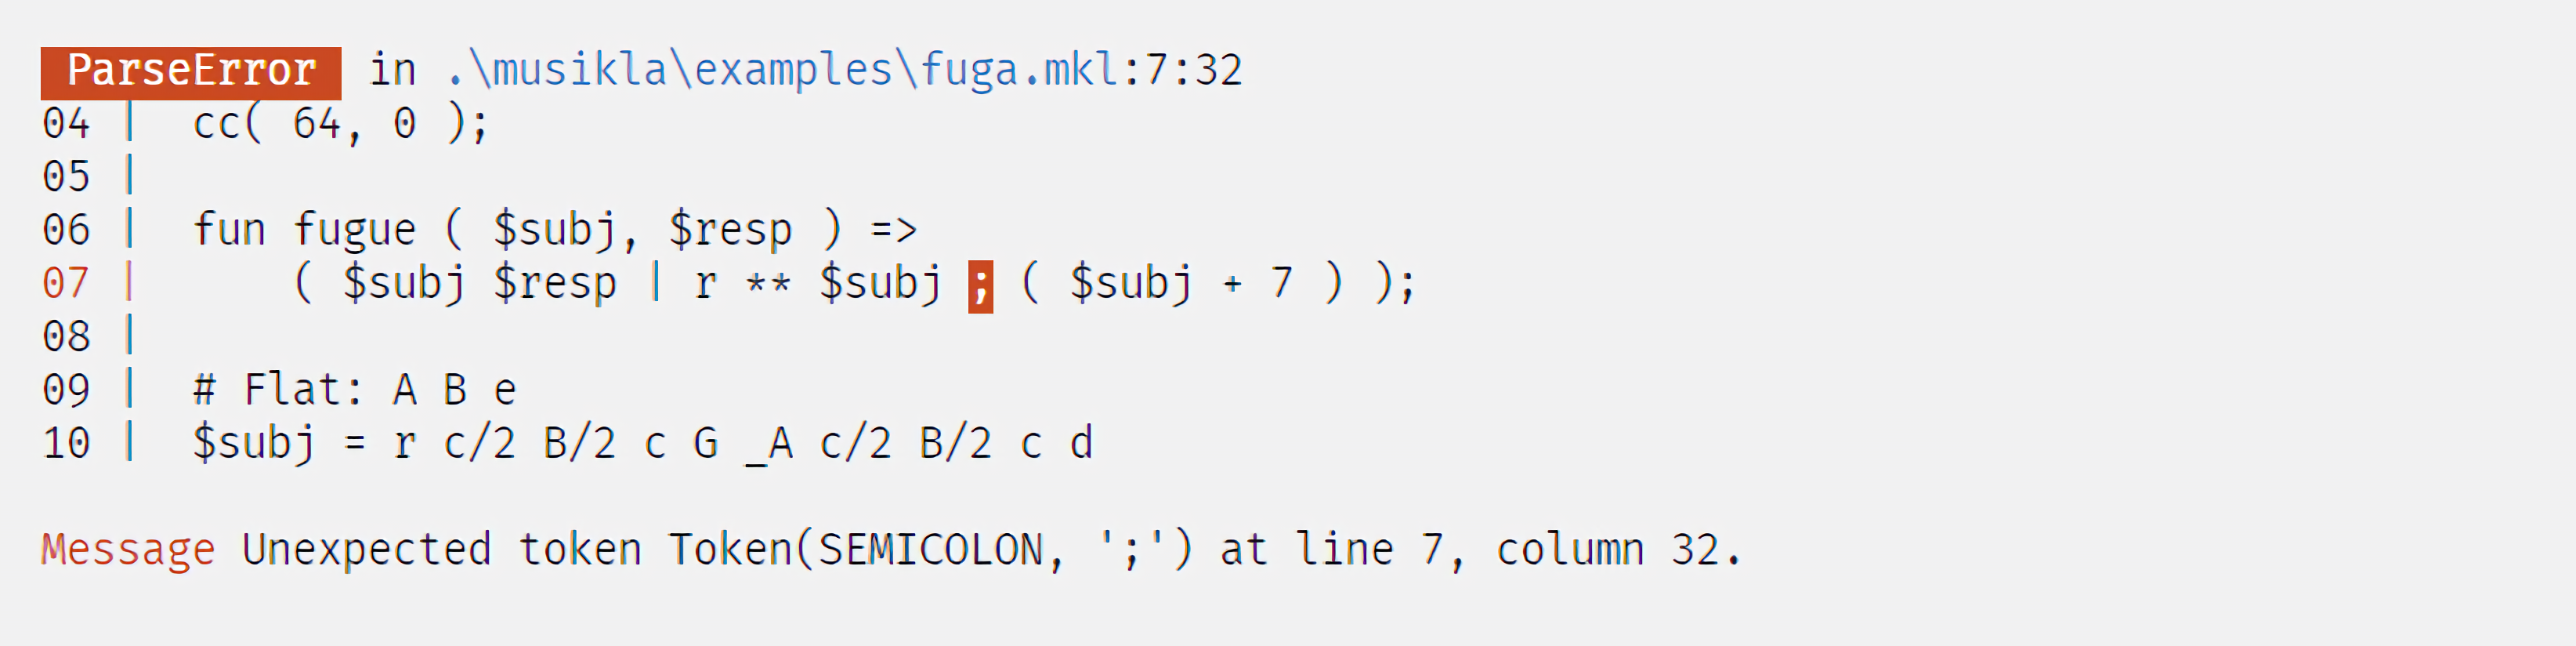
\includegraphics[width=.95\linewidth]{./img/error_reporting.png}}%
  }%
  \caption{Relatório de erro de \textit{parse}}
  \label{fig:error_reporting_parse}
\end{figure}

Para ambos os erros, o componente de relatório precisa apenas dos seguintes campos:
\begin{enumerate}
 \item[Ficheiro] Qual o caminho do ficheiro onde ocorreu o erro (opcional).
 \item[Código] O conteúdo do ficheiro que originou o erro. Este campo pode parecer redundante, tendo nós o caminho do ficheiro. Seria de esperar que podíamos simplesmente ler o ficheiro e obter o seu conteúdo. No entanto, desde o momento que o ficheiro foi lido inicialmente, e o momento em que ocorreu o erro, o seu conteúdo pode ter mudado. Por esta razão, é importante manter em memória o código dos ficheiros carregados para assegurar que os erros são mostrados corretamente.
 \item[Posição Início e Fim] Dois inteiros indicando o inicio e fim da secção contígua no ficheiro onde o erro deve ser marcado a vermelho. Podem cobrir mais do que uma linha.
 \item[Mensagem] Finalmente, qual a mensagem de erro a mostrar ao utilizador.
\end{enumerate}

\subsubsection*{Erros de Sintaxe}
Estes erros são fáceis de reportar. Sempre que há algum erro de sintaxe, o \textit{parser} emite uma exceção já com a informação da mensagem de erro, bem como a posição onde o erro ocorreu. Na nossa aplicação, só temos de tratar essa exceção, adicionando-lhe o caminho e o conteúdo do ficheiro a que estávamos a fazer \textit{parse}, e já temos toda a informação disponível para mostrar o erro.

\subsubsection*{Erros de Avaliação}
Este tipo de erros pode ocorrer em qualquer lado. Por essa razão, antes de fazer-mos \textit{parse} de qualquer ficheiro, associamos o ficheiro (e o seu conteúdo) a um inteiro único por execução. 

Depois durante a fase de \textit{parsing}, associamos a cada nó da \acrshort{ast} um triplo com três inteiros, representando o ficheiro, posição de início, e posição de fim a que esse nó corresponde.

Desta forma, no método \texttt{Node.eval()} herdado por todos os nós da \acrshort{ast}, colocamos um \texttt{try ... except ...} à volta da chamada de \texttt{Node.\_\_eval\_\_()} (função que contém o código específico de execução de cada nó). Desta forma, conseguimos adicionar a qualquer exceção que ocorra durante a execução, o triplo que o nó tem com a informação sobre o ficheiro e a sua posição no mesmo.

Esta informação é depois utilizada para preencher os campos e mostrar o relatório de erro.

\newpage

\section{Semântica Dinâmica}
As linguagens compiladas usualmente recorrem à compilação \acrfull{aot}, onde o código é transformado em código máquina antes de ser executado (durante a fase de compilação). Esta é a solução que consegue geralmente oferecer melhor \textit{performance}, menor consumo de memória e tempos de \textit{startup} mais rápido. Por outro lado, obriga a um passo de compilação separado sempre que o código fonte é alterado, e regra geral necessita de tipos de dados estáticos para melhor tirar partido das vantagens de \textit{performance}.

No que toca a linguagens interpretadas temos mais opções. Podemos então dividir os seus modos de execução em três categorias distintas, cada uma com possíveis vantagens e desvantagens, bem como diferenças na dificuldade de implementação que são bastante salientes.
\begin{description}
 \item[Interpretadores] Também chamados por vezes como interpretadores \textit{tree walk}, são usualmente os mais simples de implementar (mas também os mais lentos a executar). O seu conceito baseia-se no \textit{design pattern} homónimo, em que as operações da linguagem são modeladas numa árvore, geralmente igual ou similar à estrutura da \acrshort{ast}. Para executar uma expressão é chamado um método na raiz da árvore, e esse método irá chamar recursivamente os métodos das suas sub-expressões, passando o estado como argumentos da função, e recebendo o resultado pelo valor retornado da função.
 \item[Bytecode VM] São chamadas máquinas virtuais (VM) porque o seu comportamento assemelha-se mais ao comportamento dos processadores reais dos computadores. As expressões da árvore de sintaxe abstrata são previamente convertidas numa sequência linear de instruções mais simples (geralmente compactadas em binário para melhor \textit{performance}), também referidas como \textit{bytecode}. Cada instrução é depois executada dentro de um ciclo. Esta solução fornece um balanço entre facilidade de implementação e velocidade de execução (evitando a grande quantidade de chamadas recursivas de funções presentes nos interpretadores \textit{tree walk}).
 \item[Just In Time] O método mais complexo (mas também o que oferece melhor \textit{performance} para tarefas pesadas). O código é executado inicialmente por um dos dois métodos anteriores, de modo a recolher estatísticas sobre qual o tipo de execução mais comum do código. Após esta recolha, é gerado código máquina otimizado para os tipos de dados mais comuns de uma variável, ou para os caminhos de execução mais prevalentes, para que seja possível da próxima vez que o mesmo pedaço de código seja executado, isso ocorra com recurso ao código máquina. Este processo é geralmente repetido ao longo da execução do programa, sendo que caso a versão de código máquina gerada fique desatualizado (o tipo de dados usualmente passados a uma função mudem), essa porção de código seja invalidada e eventualmente substituída por uma nova versão mais adequada.
 \end{description}

 É possível ver que a solução ideal seria sempre a compilação \acrfull{jit}, que evita uma fase de compilação explícita e forçada ao utilizador, mas ao mesmo tempo consegue fornecer \textit{performance} competitiva para tarefas mais exigentes. No entanto é inevitável concluir que esta solução impõe custos de desenvolvimento astronómicos, e implica equipas de grande dimensão e tempos de desenvolvimento extremamente longos.
 
 Desta forma a nossa escolha reside logicamente entre a solução de \textbf{Interpretador} e uma simples \textbf{Bytecode VM}. Acabamos por escolher a primeira opção pelas seguintes razões:
 \begin{itemize}
  \item A geração de eventos músicais é relativamente barata em termos computacionais (mesmo admitindo algumas dezenas de eventos músicais por segundo).
  \item A componente mais pesada geralmente reside na sintetização dos eventos músicais (\textit{note on, note off}) em \textit{streams} de audio, mas esta tarefa é encaminhada para bibliotecas mais optimizadas e desenvolvidas em linguagens de baixo nível.
  \item A possibilidade de correr código \textit{Python} em qualquer parte da nossa linguagem já fornece um bom meio termo para quando é necessária mais alguma \textit{performance} em caminhos de execução críticos (\textit{hot paths}), sem sacrificar demasiado a simplicidade de uma linguagem destinada primariamente a músicos e não engenheiros informáticos.
  \item Também a facilidade de implementação de um interpretador significou uma velocidade ordens de magnitude superior do que seria possível de outra forma, durante a implementação da linguagem e da prototipação de funcionalidades.
  \item Uma posterior modificação do interpretador para uma \textit{bytecode VM} mais eficiente seria possível estando a linguagem mais estabilizada, e seria simples manter uma \acrshort{api} virtualmente 100\% compatível.
 \end{itemize}

 Em conclusão, cada operação foi implementada através de um método \texttt{eval()} em cada classe da \acrshort{ast}, recebendo uma variável de contexto como \textit{input}, e usando depois o valor retornado pela função como resultado da avaliação da expressão.
 
\subsection{Contexto}
A variável de contexto guarda o estado da execução, e deve conter toda a informação necessária para cada instrução poder executar. Os seus conteúdos podem ser divididos em três componentes:
\begin{description}
 \item[Timestamp] Esta propriedade é um simples inteiro que permite às expressões de geração de eventos musicais saberem qual o tempo virtual atual. Este tempo virtual é manipulado pelos vários operadores. O operador sequencial por exemplo, que recebe uma lista de expressões e emite uma lista de eventos musicais uns a seguir aos outros, avança este cursor para o fim do último evento antes de passar o contexto para avaliar a expressão seguinte.
 \item[Voz] Objeto que contém as várias propriedades musicais que devem ser aplicadas durante a geração de eventos, tais como a duração base das notas, o compasso ou as batidas por minuto.
 \item[Símbolos] Um contentor que permite aceder e modificar os símbolos disponíveis na linguagem (tais como variáveis e funções).
 \end{description}
 
 Os contextos foram desenhados com o intuito de serem leves, daí apenas conterem  referências para três variáveis. Desta forma é possível criar cópias dos contextos e permitir que operações variadas estejam a executar ao mesmo tempo com diferentes contextos.
 
 Para percebermos a razão desta necessidade, basta pensarmos no operador paralelo. Se colocarmos duas expressões musicais que devem tocar ao mesmo tempo, a geração de uma (ou mais) notas na primeira expressão não deve afetar o \texttt{timestamp} da segunda. Para isto, cada uma das expressões deve receber uma cópia do contexto (com o \textit{timestamp} inicial igual). Quando as duas expressões terminarem, no entanto, é importante que o contexto original (que gerou as duas cópias) atualize os seu \textit{timestamp} para qual for a expressão mais longa.
 
 Se prestarmos atenção, podemos estar aqui a detetar um padrão bastante comum na área da programação: o modelo \textbf{fork-join}.
 
 Apesar de estarmos a lidar com notas e eventos musicais, fundamentalmente estamos a criar ramos paralelos de execução, e queremos no final aguardar o seu resultado e uníficá-lo com o ramo original. Se substituirmos ramo por \textit{thread} para o caso da programação, ou \textit{contexto} para o nosso caso, vemos a equivalência entre os conceitos.
 
 Como tal, para além do estado (as três variáveis) que o objeto de contexto engloba, este providencia também algumas operações bastante simples e úteis:
 
 \begin{description}
  \item[Fork] Cria uma cópia do contexto, podendo receber opcionalmente também um inteiro como argumento com vista a substituir o valor do \textit{timestamp} do contexto pai. Como segundo argumento pode também receber um novo \textit{scope} de símbolos, algo que iremos aprofundar mais no capítulo seguinte.
  \item[Join] Recebe uma lista de contextos como argumento, e avança o \textit{timestamp} para o maior encontrado nessa lista.
  \item[Seek] A operação de mudar o \textit{timestamp} do contexto atual.
 \end{description}

 Os contextos não têm (nem precisam) de referências para outros \textit{contextos-pai} ou \textit{contextos-filhos}, de modo a que não é preciso grandes preocupações relativamente a fugas de memória com a criação de novos contextos: apenas são mantidos em memória os contextos que têm referências para eles, e que portanto estão ainda em uso.

\subsection{Scope de Símbolos}
Cada contexto tem uma referência para o \textit{scope} de símbolos a que tem acesso. Nestes scopes são guardadas as variáveis e funções que o utilizador (e as bibliotecas standard da linguagem) declararem. Mais uma vez, cada objeto de \textit{scope} é composto por três propriedades: uma referência ao seu \textbf{antecessor} (ou pai), uma tabela de \textit{hash} com os \textbf{símbolos}, e uma \textit{flag} booleana para designar este \textit{scope} como \textbf{opaco}.

O próprio conceito de \textit{scope} implica por si só uma hierarquia, e de facto cada objeto \textit{scope} guarda uma referência para o seu parente (ou para o valor nulo, caso seja o \textit{scope} raiz). Esta propriedade é utilizada para as operações disponíveis, tanto para pesquisar, como para atribuir valores a símbolos do \textit{scope} atual, algo que iremos verificar mais a seguir.

\begin{description}
 \item[Pesquisa] A operação de pesquisa por um símbolo começa por procurar o símbolo no próprio \textit{scope}, e caso não encontre nada, navega recursivamente para o \textit{scope} pai para efetuar a pesquisa.
 
 \item[Atribuição] A operação de atribuição segue a mesma filosofia da operação de pesquisa, procurando o \textit{scope} onde o símbolo a atribuir está guardado. No entanto, esta pesquisa decorre até encontrar o primeiro \textit{scope} opaco. Um \textit{scope} opaco não impede a leitura de valores de \textit{scopes} superiores, mas impede a escrita. Por exemplo, uma atribuição dentro de uma função cria apenas uma variável dentro do \textit{scope} dessa função.
 
 Se encontrar o símbolo nalgum \textit{scope}, então muda o seu valor nesse \textit{scope} onde está declarado. Caso contrário, é criado um novo símbolo no \textit{scope} original onde a operação de atribuição foi iniciada.
 
 \item[Enumeração] A operação de enumeração permite listar quais os símbolos visíveis a partir de um \textit{scope}. Ela permite listar não só os símbolos do próprio \textit{scope}, mas também dos seus pais, tendo o cuidado para não retornar símbolos que tenham sido obscurecidos por um \textit{scope} mais em baixo. Esta é útil para importar símbolos do \textit{scope} de um módulo para outro, ou para implementar funcionalidades como \textit{autocomplete} sobre um script em execução (e permitir sugerir os símbolos disponíveis).
 
 \item[Apontadores] Como vimos na atribuição, é impossível alterar valores de variáveis globais dentro de \textit{scopes} opacos (como dentro de funções, por exemplo). Para colmatar isso, similar ao operador \texttt{global} e \texttt{nonlocal} do \textit{Python}, é possível instruir um \textit{scope} a criar um apontador para um símbolo declarado noutro \textit{scope}, de forma a que quando ocorre alguma atribuição, a alteração é replicada no seu \textit{scope} original.
\end{description}

\subsection{Módulos}
O Musikla dispõe também da possibilidade de executar código separado em vários ficheiros, cada um sendo considerado um módulo. O utilizador pode configurar uma lista de pastas (num conceito similar à variável de ambiente \texttt{\$PATH}) onde serão procurados módulos quando alguma instrução \texttt{import} é avaliada. Também é possível passar um caminho absoluto ou relativo ao módulo que iniciou a importação.

Cada ficheiro importado é executado apenas uma vez durante a primeira importação, e no final o seu \textit{scope} é guardado em \textit{cache} para ser usado em futuras importações.

Cada instrução de importação é dividida em duas fases: primeiro, o caminho passado é resolvido no caminho real e absoluto do ficheiro. Só depois é verificada na \textit{cache} se o ficheiro já foi importado antes. Uma vez obtido o seu \textit{scope}, os seus símbolos são enumerados e copiados para o \textit{scope} que efetuou a importação (com símbolos que comecem com um \textit{underscore} sendo tratados como símbolos privados e ignorados).

Para isso, quando o interpretador é inicializado, é criado um \textit{scope} raiz chamado \textbf{prelude}, e um \textit{scope} filho. Cada módulo importado é executado num \textit{scope} criado sempre a partir do \textit{prelude}. Desta forma, os símbolos aí guardados estão sempre acessíveis em todos os módulos importados.

% TODO Imagem a exemplificar os scopes

\subsection{Operadores Musicais}
A sintaxe suporta os operadores aritméticos e de comparação usuais nas linguagens de programação. De modo geral, a sua sintaxe e semântica na nossa linguagem, o que seria expectável para cada um deles, pelo que não vale enumerá-los a todos nesta secção. No entanto, existem alguns operadores menos convencionais, ou até \textit{overloads} de operadores convencionais (como o operador de multiplicação e adição) que funcionam de forma diferente quando empregues junto a valores do tipo musical. São esses os casos que iremos abordar nas seguintes sub-secções.

Um aspeto importante a ter em conta é que estes operadores não estão restritos gramaticalmente para aceitar apenas expressões musicais, mas aceita sim qualquer tipo de expressão. O seu tipo (e portanto a sua semântica) são apenas decididos em \textit{runtime} (imitando o modo de funcionamento do \textit{overloading} de operadores em \textit{Python}). Isto é necessário porque uma variável pode conter tanto um número como uma expressão musical, e o seu verdadeiro valor apenas é conhecido em execução.

\subsubsection{Sequencial/Concatenação}
Ao longo deste documento já vimos várias instâncias de como declarar uma nota ou um acorde. O ato de concatenar esses eventos (ou seja, reproduzi-los em sequência) é tão fundamental para a linguagem que também é algo que já vimos inúmeras vezes nos exemplos sem pensar muito nisso. Uma das razões para isso deve-se à sua sintaxe (ou falta dela, na verdade). O ato de concatenar eventos musicais é tão simples como escrevê-los uns à frente dos outros, sem nenhum tipo de separador especial (para além dos opcionais espaços em branco). O evento ficam com o seu tempo inicial sempre igual ao tempo final do evento anterior.

\begin{lstlisting}[caption={Excerto da música \textit{Wet Hands} de C418},label=lst:ops-concat,belowcaptionskip=-\medskipamount]
S4/4 T74 L/8 V90;
A, E A B ^c B A E D ^F ^c e ^c A3;
\end{lstlisting}


\begin{figure}[ht]
  \centering
  {%
  \setlength{\fboxsep}{0pt}%
  \setlength{\fboxrule}{0pt}%
  \fbox{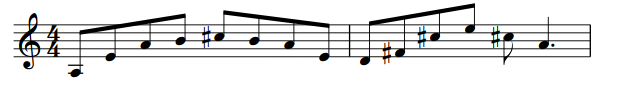
\includegraphics[width=.85\linewidth]{../../code/musikla/musikla/examples/paper/concatenation2.png}}%
  }%
  \caption{Pauta musical gerada pela linguagem\protect\footnotemark, versão áudio disponível \href{https://drive.google.com/open?id=1TP4lcul81s8iMCUFmD3HKnSpeftCzKT0}{\underline{aqui}}\protect\footnotemark.}
  \label{fig:ops-concat}
\end{figure}

\footnotetext[\numexpr\thefootnote-1]{Renderizado com a biblioteca \$ABC\_UI, com alguns ajustes manuais feitos para melhorar a clareza.}
\footnotetext{Concatenação \url{https://drive.google.com/open?id=1TP4lcul81s8iMCUFmD3HKnSpeftCzKT0}}

Também é importante salientar o facto de que as listas de instruções (\textit{statements}) seguem a mesma semântica do operador de concatenação. Cada linha só vai tocar as suas notas quando as linhas anteriores tiverem acabado. Neste exemplo portanto, ter tudo na mesma linha ou separado em duas (ou mais) tem o mesmo resultado, variando apenas a legibilidade.

\subsubsection{Repetição}
O operador de repetição é bastante similar ao operador de concatenação. E faz sentido, uma vez que repetir uma expressão musical $N$ vezes pode ser pensado como um caso particular da concatenação onde existem $N$ operandos, todos iguais, uns em frente aos outros.

\begin{lstlisting}[caption={Excerto do começo do tema principal de Westworld, por Ramin Djawadi},label=lst:ops-repetition,belowcaptionskip=-\medskipamount]
I1 S6/8 T140 L/8 V90;
A*11 G F*12
\end{lstlisting}

\begin{figure}[ht]
  \centering
  {%
  \setlength{\fboxsep}{0pt}%
  \setlength{\fboxrule}{0pt}%
  \fbox{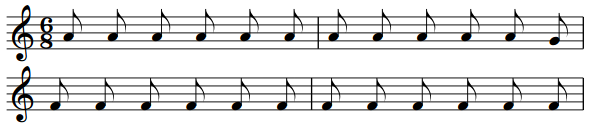
\includegraphics[width=.85\linewidth]{../../code/musikla/musikla/examples/paper/repetition2.png}}%
  }%
  \caption{Pauta musical gerada pela linguagem, versão áudio disponível \href{https://drive.google.com/open?id=1IIm8PQkLsNFMK9MNSVubJSG6SP6KwhPL}{\underline{aqui}}\protect\footnotemark.}
  \label{fig:ops-repetition}
\end{figure}

\footnotetext{Repetição \url{https://drive.google.com/open?id=1IIm8PQkLsNFMK9MNSVubJSG6SP6KwhPL}}

Este operador, apesar de bastante simples, é também bastante útil para repetir pequenos acompanhamentos (mesmo notas singulares) muitas vezes, ou até para repetir poucas vezes acompanhamentos mais complexos. Evitando repetir os acompanhamentos no código, é possível efetuar alterações em apenas um sítio e ver essas alterações repetirem-se ao longo de toda a estrutura musical.

\subsubsection{Paralelo}
O operador paralelo permite reproduzir múltiplas sequências de eventos musicais em paralelo. Podemos dizer que conceptualmente, o operador paralelo é uma função que recebe uma lista de sequências musicais, e retorna uma única sequência com todas as sequencias combinadas. No entanto é importante que lembrar que o operador tem de respeitar os princípios de \textit{\textbf{lazyness}} (não pedir mais eventos de cada vez do que o que os que são estritamente necessários) e \textbf{ordem} (a sequência de eventos resultantes tem de estar estritamente ordenada pelo tempo de início de cada evento).

\begin{lstlisting}[caption={Excerto da música \textit{Soft to Be Strong} de Marina},label=lst:ops-parallel,belowcaptionskip=-\medskipamount]
T120 V70 L1;
r/4 ^g/4 ^g/4 ^g/4   ^f/2 e/8 ^d3/8   ^c2 | [^Cm] [BM]  [AM] [BM] 
\end{lstlisting}

\begin{figure}[ht]
  \centering
  {%
  \setlength{\fboxsep}{0pt}%
  \setlength{\fboxrule}{0pt}%
  \fbox{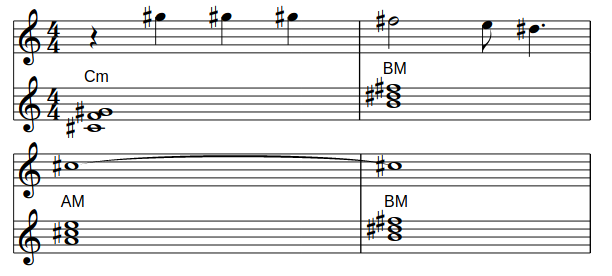
\includegraphics[width=.85\linewidth]{../../code/musikla/musikla/examples/paper/parallel2.png}}%
  }%
  \caption{Pauta musical gerada pela linguagem, versão áudio disponível \href{https://drive.google.com/open?id=1ENTm3hZonYHyQIOgRZ8TQ1Qz-AfRLt2I}{\underline{aqui}}\protect\footnotemark.}
  \label{fig:ops-parallel}
\end{figure}
\footnotetext{Paralelo \url{https://drive.google.com/open?id=1ENTm3hZonYHyQIOgRZ8TQ1Qz-AfRLt2I}}

A implementação do operador paralelo depende de um simples algoritmo de \textit{merge sorted} (não relacionado com o conhecido algoritmo de ordenação de \textit{arrays merge sort} inventado por John von Neumann).

A função \textit{merge sorted} recebe $N$ operandos e cria um \textit{buffer} também de tamanho $N$. Para cada operando, ela cria um \textit{fork} do seu contexto, para que cada operando possa executar concorrentemente e assim modificar apenas o seu próprio contexto. Depois, ainda durante a inicialização do algoritmo, a função pede a cada operando um evento (que são guardados nas respetivas posições do \textit{buffer}).

Após o \textit{buffer} estar preenchido pela primeira vez com um evento por operando, o algoritmo procura o evento mais recente (o evento com \textit{timestamp} menor) guardado no \textit{buffer}. Vamos assumir que esse evento se encontra guardado na posição $K$ do \textit{buffer}, sendo $k < N$. O método emite esse evento \texttt{buffer[K]} para a sequência músical de saída, e de seguida pede ao operando na posição $K$ o seu próximo evento, usando-o para substituir o que estava anteriormente no \textit{buffer} nessa mesma posição (guardando o valor \texttt{null} caso o operando $K$ já tenha chegado ao fim). O algoritmo repete depois este passo até todos os operandos terem chegado ao fim.

\subsubsection{Transposição}
As operações \verb|Music + Integer| e \verb|Music - Integer| correspondem à transposição de notas (e acordes). Podem ser aplicados a notas singulares ou expressões musicais complexas, o que resulta na transposição a ser aplicada a cada uma das notas da expressão musical.

\begin{lstlisting}[caption={Exemplo de transposição de um acompanhamento com três notas},label=lst:ops-transpose,belowcaptionskip=-\medskipamount]
L/8;
(A B c) (A B c) + 12;
\end{lstlisting}

\begin{figure}[ht]
  \centering
  {%
  \setlength{\fboxsep}{0pt}%
  \setlength{\fboxrule}{0pt}%
  \fbox{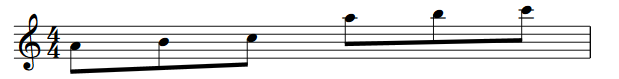
\includegraphics[width=.85\linewidth]{../../code/musikla/musikla/examples/dissertation/transpose.png}}%
  }%
  \caption{Pauta musical gerada pela linguagem, versão áudio dísponível \href{https://drive.google.com/file/d/1xVey6on6Q-sWjNgo__Llb3QgOF1-_axa}{\underline{aqui}}\protect\footnotemark.}
  \label{fig:ops-transpose}
\end{figure}
\footnotetext{Transposição \url{https://drive.google.com/file/d/1xVey6on6Q-sWjNgo__Llb3QgOF1-_axa}}

Neste simples exemplo listado em \ref{lst:ops-transpose} e ilustrado em forma de pauta musical na Figura \ref{fig:ops-transpose}, podemos ver claramente que a música é composta por dois triplos de notas, ambos com o mesmo padrão, sendo a única diferença que o segundo é tocado uma oitava acima (12 semitons).

\subsubsection{Arpeggio}
A operação \verb|Chord * Music| \footnote{Na implementação atual, o operador aceita não só acordes como primeiro operando, mas qualquer expressão musical} permite aplicar um \textbf{Arpeggio}. Esta operação consiste em pegar nas notas presentes no primeiro operador e colocá-las numa lista de $0 .. N$ não inclusivo (sendo $N$ o número de notas no acorde). De seguida é avaliada a segunda expressão musical, mantendo os seus tempos e posições, mas substituindo as notas pelas pertencentes ao acorde. O modo de substituição usa a seguinte escala: \texttt{C D E F G A B}. Isto é, assume a nota \texttt{C} como base (a que é substituída pela primeira nota do acorde), a nota \texttt{D} sendo substituída pela segunda nota do acorde, e por aí fora.

\begin{lstlisting}[caption={Três acordes diferentes arpegiados com o mesmo padrão},label=lst:ops-arpeggio,belowcaptionskip=-\medskipamount]
S4/4 L/8 T85;

$p = C D E D2 E C2;

[CeG]*$p [Ac'e]*$p [Fac]*$p [CeG]*$p;
\end{lstlisting}

\begin{figure}[ht]
  \centering
  {%
  \setlength{\fboxsep}{0pt}%
  \setlength{\fboxrule}{0pt}%
  \fbox{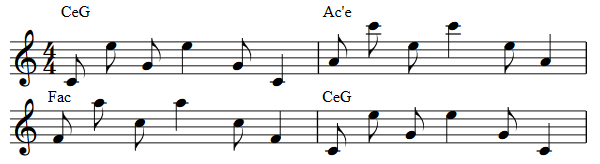
\includegraphics[width=.85\linewidth]{../../code/musikla/musikla/examples/dissertation/arpeggio.png}}%
  }%
  \caption{Pauta musical gerada pela linguagem, versão aúdio dísponível \href{https://drive.google.com/file/d/1E6ayR6gG2CfsikWFHijnEIui0rR1cAL7}{\underline{aqui}}\protect\footnotemark.}
  \label{fig:ops-arpeggio}
\end{figure}
\footnotetext{\textit{Arpeggio} \url{https://drive.google.com/file/d/1E6ayR6gG2CfsikWFHijnEIui0rR1cAL7}}

No exemplo da listagem \ref{lst:ops-arpeggio} recorremos ao uso de uma variável para guardar o padrão da nossa melodia. De seguida usamos o operador de \textit{arpeggio} em cada um dos acordes, sempre com o mesmo padrão. Esta funcionalidade permite definir uma melodia e testar rapidamente múltiplas variações da mesma sem ter de alterar manualmente a melodia de cada vez.

Atualmente a definição do padrão recorre à sintaxe das músicas usuais, por conveniência. No futuro, seria interessante implementar uma sintaxe específica para a definição de \textit{arpeggios}, usando por exemplo numeração romana. Dessa forma, o padrão do exemplo na listagem \ref{lst:ops-arpeggio} ficaria algo como \verb|I II III II2 III I2|. Outra possibilidade seria a de usar a numeração decimal, com alguma marcação para distinguir dos números inteiros, tal como \verb|1º 2º 3º 2º2 3º 1º2|.


\subsubsection{Redimensionamento}
O operador de \textbf{Redimensionamento}, denotado pela sintaxe \verb|Music ** Integer|, \verb|Music ** Fraction|, ou \verb|Music ** Music|, pode talvez ser o menos intuitivo, mas é algo bastante útil. Ele permite mudar o tamanho de uma expressão arbitrária já declarada, para combinar com outra duração expressa num inteiro, fração, ou inferida através da duração de uma segunda expressão musical. O seu valor de retorno é então o primeiro operando, mas com os tempos proporcionalmente esticados (ou encolhidos) de modo a, no total, ficarem com a nova duração escolhida.

\begin{lstlisting}[caption={Redimensionamento da duração de uma expressão músical},label=lst:ops-retime,belowcaptionskip=-\medskipamount]
S2/4 L/8 T90;

$chords = V90 [CeG] [Ac'e] [Fac] [CeG];
$melody = CGde2gc2 CGdr5;

$chords ** $melody | $melody;
\end{lstlisting}

\begin{figure}[ht]
  \centering
  {%
  \setlength{\fboxsep}{0pt}%
  \setlength{\fboxrule}{0pt}%
  \fbox{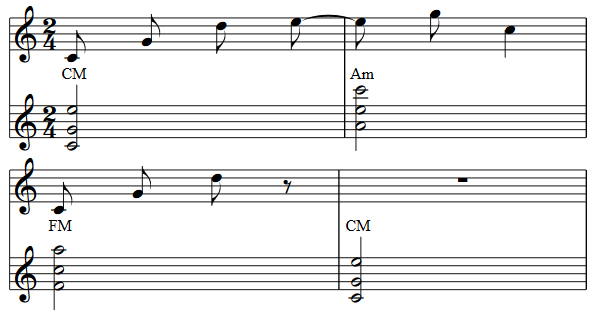
\includegraphics[width=.85\linewidth]{../../code/musikla/musikla/examples/dissertation/retime.png}}%
  }%
  \caption{Pauta músical gerada pela linguagem, versão aúdio dísponível \href{https://drive.google.com/file/d/1aVVXGDVQEAmHl-jadSnZ6OqIGmgqhgxR}{\underline{aqui}}\protect\footnotemark.}
  \label{fig:ops-retime}
\end{figure}
\footnotetext{Redimensionamento \url{https://drive.google.com/file/d/1aVVXGDVQEAmHl-jadSnZ6OqIGmgqhgxR}}

No exemplo presente na listagem \ref{lst:ops-retime}, temos duas variáveis com durações diferentes. A primeira, \textbf{\texttt{\$chords}}, tem a duração total de \textbf{$\frac{1}{2}$} ($4 \times \frac{1}{8}$). Por sua vez, a segunda variável, \textbf{\texttt{\$melody}}, tem a duração de \textbf{2} ($16 \times \frac{1}{8}$). As duas durações podiam ser ajustadas manualmente (bastando multiplicar a duração de cada acorde por 4), mas isso implicava que qualquer mudança na melodia exigia recalcular as proporções manualmente. E também nem todas as situações apresentam contas tão simples como $2 \div \frac{1}{2}$. Deste modo, os cálculos são feitos automaticamente pela aplicação e estão sempre atualizadas.

\section{Biblioteca Standard}
A biblioteca \textit{standard} que é incluída com o interpretador Musikla foi também um dos grandes desafios do desenvolvimento deste projeto. Obviamente, o seu desenvolvimento ocorreu de uma forma faseada, ao mesmo tempo que a linguagem e o interpretador eram desenvolvidos. Isso significa que desenvolver a biblioteca não é apenas a tarefa de adicionar novas funcionalidades, mas também de reescrever ou adaptar functionalidades existentes que tenham sido adicionadas numa fase inicial do desenvolvimento da linguagem. Por essa razão as suas interfaces públicas podiam estar desenhadas à volta de uma linguagem que tinha menos funcionalidades que a versão atual, sejam elas objetos, listas ou passagem de argumentos com nome.

No diagrama abaixo podemos ver uma lista dos módulos que são disponibilizados pela linguagem. As funções e classes listadas abaixo são apenas um pequeno exemplo do que é implementado na biblioteca. A documentação mais completa pode ser encontrada \href{https://pedromsilvapt.github.io/miei-dissertation/}{online}.

\begin{figure}[h]
\begin{center}
    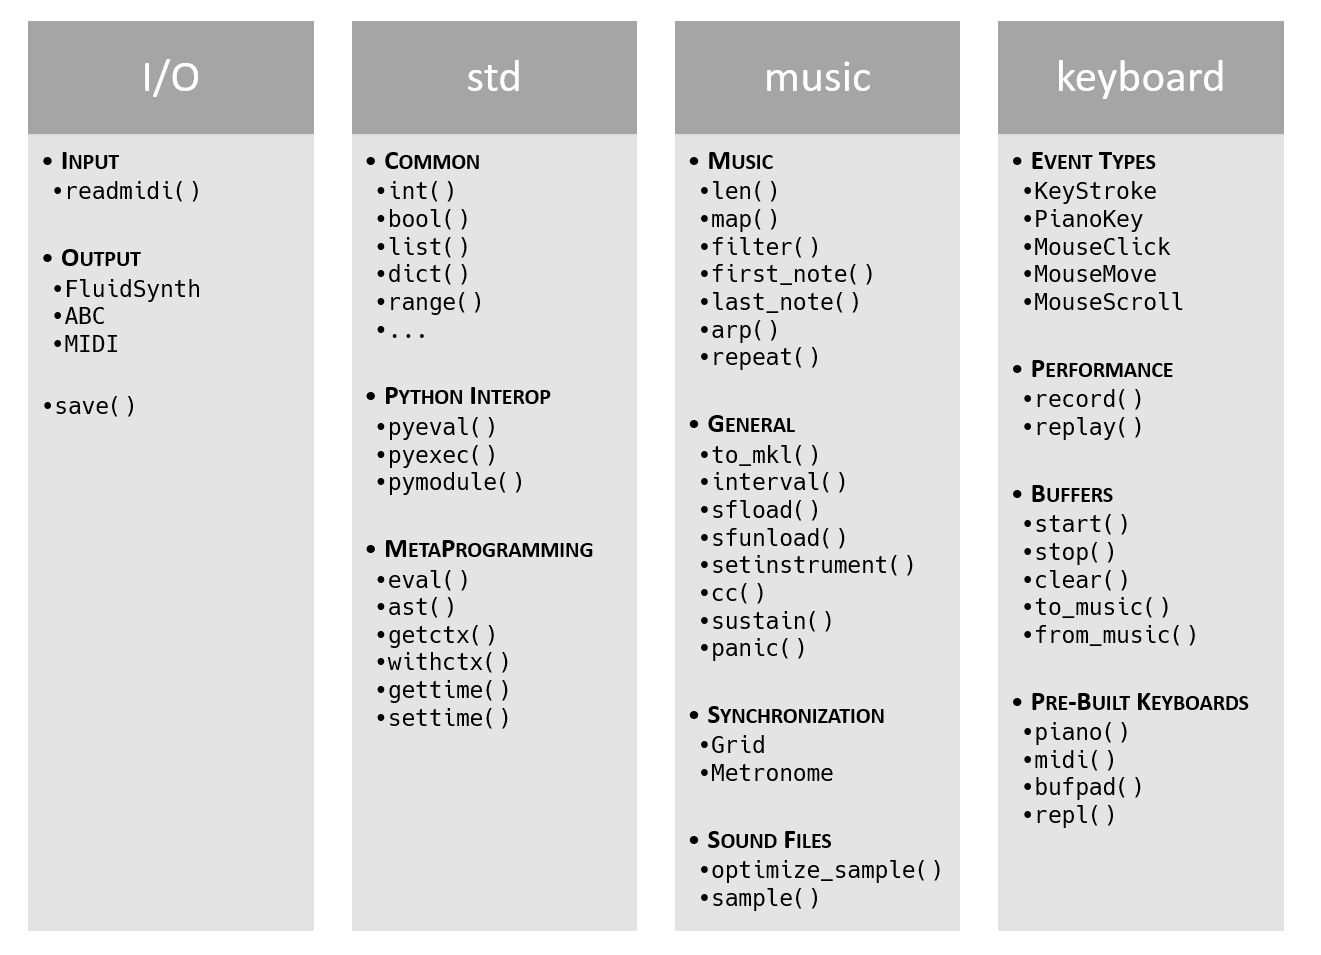
\includegraphics[width=0.87\textwidth]{img/standard_library.png}
\end{center}
\caption{Organização do projeto}
\end{figure}

Todos estes módulos, por serem tão comuns e essenciais, são sempre carregados automaticamente antes de executar um \textit{script} Musikla, pelo que não há necessidade de os importar manualmente.

\subsection{Inputs \& Outputs}
Durante a execução, os eventos musicais são representados em memória por objetos \textit{Python} que derivam da classe base \textbf{MusicEvent}, e estão agrupados em sequências pelos objetos que derivam da classe \textbf{Music}.

A forma mais óbvia de criar estes objetos é utilizando a sintaxe de literais de música inspirada pelo projeto \textit{abc notation} que pode ser utilizada dentro da própria linguagem.

No entanto, não há nenhuma restrição que force este a ser o único método de introdução ou geração de eventos musicais. De facto, existem já vários formatos de descrição de música, e a capacidade de os poder ler e traduzir para objetos musicais dentro da nossa linguagem, indistinguíveis daqueles que são criados pela sintaxe de literais, traz inúmeras vantagens e abre a possibilidade de este projeto se tornar como um canivete suíço da notação musical, capaz de ler, transformar e depois também escrever em diversos formatos diferentes.

Para além de ser capaz de ler (\textbf{input}) eventos musicais e transforma-los nos objetos em memória que a nossa linguagem expecta, é também importante poder, depois de os criar e transformar ao nosso gosto, poder fazer algo de útil com eles. Ou seja, escrever (\textbf{output}) estes eventos musicais em diversos formatos.

O verdadeiro objetivo da linguagem é que seja extensível, de modo a que qualquer pessoa capaz de programar \textit{Python} possa conectar um novo \textit{input} ou \textit{output} para as suas necessidades específicas, sem necessitar de ter conhecimentos intrínsecos do funcionamento de toda a linguagem. Nesta secção iremos descrever alguns dos modos de \textit{input} e \textit{output} incluídos de base com a linguagem e que servem de prova de conceito do que é possível fazer com ela.

Os \textit{outputs} podem ser globais, ou seja, aplicarem-se aos eventos emitidos pela aplicação. Neste caso são geralmente passados como argumentos de linha de comandos, ou adicionados durante a execução através da função \texttt{\$script::player::add\_sequencer()}. Também é possível gravar apenas expressões de música específicas com a função \texttt{save()}.
\subsubsection{FluidSynth}
Esta biblioteca serve apenas como \textbf{output} para a linguagem, e permite sintetizar sons a partir de ficheiros \textit{SoundFont}. Os sons gerados podem depois ser passados diretamente para as colunas do computador, ou guardados em disco num ficheiro de música.

Para implementar este \textit{output}, utilizamos o projeto \textit{pyfluidsynth}\cite{pyfluidsynth} para interoperar o nosso código \textit{Python} com a biblioteca \textit{FluidSynth}, escrita em \textit{C}. Como os \textit{bindings} do projeto em \textit{Python} não cobriam toda a \acrshort{api} da biblioteca que nós necessitávamos, optamos por realizar um \textit{fork} dos \textit{bindings}, o que nos permitiu depois efetuar as alterações necessárias à nossa medida.

O objeto principal disponibilizado pelo \textit{FluidSynth} é o objeto \texttt{Synth}. Este disponibiliza inúmeros métodos (baseados no \textit{standard} MIDI) para ativar e desativar uma nota, mudar o instrumento, definir o valor de um controlo, entre muitas outras. Os métodos chamados neste objetos são aplicados imediatamente, pelo que se tivermos uma lista de ações (eventos musicais) a tomar com \textit{timestamps} variados, temos de tratar do seu correto agendamento.

Felizmente a biblioteca também providencia um objeto para isso: \texttt{Sequencer}.  Para o efeito registamos um \textit{callback} na nossa aplicação que recebe o evento e é responsável por o aplicar ao \texttt{Synth}. Depois, sempre que algum evento é gerado, chamamos a função \texttt{Sequencer.timer()} e passamos-lhe o \textit{timestamp} em que deve ser executado o evento, bem como o evento em si e o \textit{callback} a chamar quando o temporizador concluir. Uma das vantagens é o facto de o FluidSynth já disponibilizar uma interface segura de acesso entre \textit{threads}\cite{henningsson2011fluidsynth}.

A maioria dos eventos da nossa linguagem são inspirados pelo \textit{standard} MIDI, tal como a é desenhada a \acrshort{api} do sintetizador do \textit{FluiSynth}, pelo que aplicação dos eventos passa geralmente apenas por chamar a função correta e fornecer-lhe os parâmetros carregados pelo evento. Há no entanto uma exceção à regra, algo que iremos aprofundar mais à frente, e que é a possibilidade de reproduzir, para além de notas musicais, mas ficheiros musicais também. Infelizmente o \textit{FluidSynth} não suporta diretamente este tipo de utilização, mas com alguma criatividade foi possível implementá-la usando as ferramentas que nos eram disponibilizadas.

A sintetização de notas efetuada pelo \textit{FluidSynth} recorre aos ficheiros \textit{Soundfont}, que podem ser descritos de uma forma muito simplista como um dicionário que associa a cada nota de cada instrumento um \textit{buffer} contendo o som a ser reproduzido, mais algumas configurações que permitem ajustar o som gerado a diversas situações (duração da nota, velocidade, entre outras).

Estas fontes de som podem ser carregadas para o \textit{FluidSynth} e através do método \texttt{Synth.sfload()} e passando-lhe o caminho do ficheiro. Mas para além de fontes carregadas do disco, também é disponibilizada uma estrutura \texttt{RamSFont} que permite criar, representar e editar uma fonte de som completamente em memória, que pode ser depois associada ao sintetizador pelo método \texttt{Synth.add\_sfont()}.

Sempre que algum evento musical traz consigo um ficheiro de música para ser reproduzido, nós associamos o conteúdo desse ficheiro a uma nota de um instrumento virtual da \texttt{RamSFont} que criamos. Quando o mesmo ficheiro é pedido para ser reproduzido várias vezes, a mesma nota do mesmo instrumento é utilizada, evitando estar sempre a ler os conteúdos do ficheiro. Este evento musical é depois convertido num evento de reprodução de notas, com a informação da nota e do instrumento a usar sendo preenchidas automaticamente com o nosso instrumento virtual.

Desta forma, podemos reproduzir ficheiros arbitrários de som em conjunto com as notas musicais de uma forma transparente para o utilizador.

No entanto, um obstáculo que encontramos durante a implementação desta funcionalidade foi o facto de os sons associados a notas com um valor inteiro inferior a 15 (cada instrumento pode ter 128 notas, entre 0-127) tinham o seu \textit{pitch} distorcido, mesmo quando eram passadas as \textit{flags} para que os sons fossem reproduzidos sem ajustamento do \textit{pitch}. Este comportamento no entanto desaparecia acima de notas com o valor 15, pelo que adotamos esse valor como a nossa base (o que desperdiça 15 lugares em cada instrumento que poderiam ser associados a sons). Como na \textit{SoundFont} podemos utilizar também vários instrumentos, isso significava que ainda assim conseguíamos reproduzir $127 \times 113 = 14351$ sons distintos, o que é bastante mais do que suficiente para a maioria dos casos.

\subsubsection{MIDI}
Mais uma biblioteca que achamos importante incluir de base foi o suporte para leitura e escrita de dados MIDI. Isto tanto pelo facto de que o \textit{standard} MIDI é um dos mais utilizados no mundo da música, mas também porque a nossa implementação da linguagem, particularmente relativa à representação dos eventos musicais em memória, foi fortemente inspirada por este formato. Dessa forma, implementar funções de transformação dos não exigiu demasiado esforço. Para o efeito, utilizamos o módulo \textit{Python} \texttt{mido}, que permite ler e escrever eventos MIDI, tanto de portas como de ficheiros em disco.

A nível de leitura (\textbf{input}), o módulo disponibiliza uma função \texttt{readmidi()} que permite ler eventos musicais de um ficheiro ou porta MIDI, retornando um objeto do tipo \textbf{Music}. A função aceita os seguintes parâmetros (sendo os parâmetros de ficheiro ou de porta mutuamente exclusivos):

\begin{description}
 \item[file] \textit{(Opcional)} Quando presente, lê os eventos musicais de um ficheiro MIDI.
 \item[port] \textit{(Opcional)} Permite ler os eventos de uma porta em vez de um ficheiro. Este parâmetro aceita vários valores.
 \begin{description}
  \item[True] Se receber este valor, tenta listar as portas MIDI disponíveis e escolher a mais indicada para ler os eventos.
  \item[List{[String]}] Uma lista de nomes de portas para escutar. Os eventos das portas referidas são combinados numa única sequência de eventos, como se viessem todos da mesma porta.
  \item[String] O nome de uma única porta para estar à escuta de eventos.
 \end{description}
 \item[voices] \textit{(Opcional)} Uma lista de vozes para mapear a cada canal MIDI a que os eventos pertencem. Quando nenhuma voz é especificada, a voz atual presente no contexto é utilizada para todos os canais.
 \item[cutoff\_sequence] \textit{(Opcional)} Uma sequência de notas ou eventos músicais que, quando recebidos pelas portas MIDI, são utilizados como sinal para terminar imediatamente a leitura e retornar a sequência de eventos já capturada. È ignorada quando a fonte de leitura é um ficheiro.
 \item[ignore\_message\_types] \textit{(Opcional)} Uma lista de \textit{strings} com os nomes de mensagens MIDI que devem ser ignoradas.
\end{description}

É também possível escrever (\textbf{output}) para portas e ficheiros MIDI de forma bastante simples. Este \textit{output} é ativado automaticamente quando se grava um ficheiro com a extensão MIDI, ou quando se prefixa o nome de uma porta com a \textit{string} \texttt{midi://}.

Ao escrever para ficheiros ou portas MIDI, é possível filtrar apenas os eventos de certas vozes, e mapear também os canais atribuídos a cada voz. Isto é extremamente útil para permitir ligar a aplicação a programas \acrshort{daw}, e permitir receber os eventos MIDI em faixas separadas (para aplicar efeitos ou transformações específicas a cada faixa).

\subsubsection{ABC}
Outro dos formatos de saída suportados é o formato \textbf{abc notation}. A sintaxe das notas e acordes da nossa linguagem é fortemente inspirada nesta notação, pelo que não seria estranho pensar que escrever para este formato não seria nada de especial. E em parte é verdade, na medida que gerar o texto com o formato certo não é complicado.

A maior diferença é, no entanto, o facto de que o formato \textit{abc} é estático, e a sua estrutura foi desenhada para imitar de certa forma a notação das partituras musicais. Tudo isto envolve conceitos como agrupar as notas por vozes, pautas, compassos, claves, entre outros. De certa maneira, o modelo de dados que a linguagem usa para representar as notas em memória mapeia-se de forma muito mais simples para o formato \textit{MIDI} do que para o \textit{abc}.

Para colmatar este facto, os eventos, antes de serem convertidos para o formato \textit{abc}, são introduzidos numa \textit{pipeline} que executa uma série de passos de modo a tornar a conversão mais simples. De grosso modo, os passos pela ordem que são executados, são os seguintes:

\begin{itemize}
 \item Em primeiro lugar o sistema tenta converter quaisquer notas que possam estar a ser emitidas como eventos \textit{on/off} separados. Isto acontece quando, por exemplo, o teclado é usado, o que pode implicar começar a tocar as notas sem saber quando o utilizador as vai parar. Os pares de eventos são então convertidos num só evento com a informação do início e da duração da nota.
 \item Em segundo lugar, o sistema tenta identificar as notas paralelas que possam estar a ser emitidas e que possam pertencer a um acorde. Isto acontece mais uma vez quando, ao invés de usar a sintaxe de acordes presente na linguagem, o usa o teclado para gerar o acorde através de notas/teclas diferentes ativadas ao mesmo tempo.
 \item Em terceiro lugar, as notas que pertençam à mesma voz mas que tenham \textit{overlap} na sua duração, são colocadas em linhas diferentes. Mais uma vez, isto acontece mais frequentemente quando o teclado é usado, onde o utilizador pode estar a tocar notas concorrentemente da forma que quiser.
 \item Em quarto lugar, são inferidos eventos pausa quando duas notas consecutivas pertencentes à mesma voz têm um intervalo. Mais uma vez, isto acontece mais frequentemente quando o utilizador toca com o teclado. Mas neste caso pode também acontecer quando as notas são declaradas pela sintaxe da linguagem, como por exemplo na seguinte situação \texttt{A ( B | C )}, onde as notas \texttt{A} e \texttt{B} ficam na mesma pauta. A nota C, no entanto, como se sobrepõe com a nota \texttt{B}, pelo passo anterior, seria movida para a sua pauta. No entanto, esta pauta não teria nada ao início, e por isso precisa de uma pausa. Seria conceptualmente equivalente ao resultado de \texttt{(A B) | (r C)}.
 \item Finalmente em quinto lugar, são introduzidos eventos especiais na sequência musical para identificar, para cada voz em separado, quando devem ser introduzidos novos compassos, ou novas pautas na partitura. Do mesmo modo, isto implica que notas e acordes cuja duração não caiba num compasso, sejam divididos quantas vezes forem necessários, e conectados através de \gls{ligaduras}.
\end{itemize}

Estas transformações são reutilizáveis (não estão fortemente acopladas ao formato \textit{abc}) e são implementadas utilizando o conceito de transformadores, que iremos abordar mais à frente neste documento.

Muitas destas transformações são, no entanto, imperfeitas por natureza: a deteção de acordes a partir de notas paralelas individuais, por exemplo, nunca pode ter 100\% de certeza se as notas que agrupou são realmente um acorde. É possível que o músico tivesse a intenção de que as várias notas pertencessem a vozes diferentes, por exemplo.

Para além disto, a notação musical é tão complexa que apenas uma pequena parte é suportada pela nossa linguagem. Deste modo, é preciso ter em mente que apesar de a linguagem ser capaz de gerar ficheiros \textit{abc} válidos, e com a sua estrutura maioritariamente correta de acordo com o que o utilizador tivesse em mente, serão muitas vezes necessários pequenos ajustes manuais para personalizar os resultados aos gostos de cada um. Ainda assim, o facto de não ser necessário escrever o ficheiro todo manualmente é por si só uma vantagem enorme.

Isto porque o ficheiro \textit{abc} não serve só como um formato de texto. Existem várias ferramentas para o converter para outros formatos, como \textit{PDF}. Por exemplo, o projeto \textbf{\$ABC\_UI}\footnote{\url{http://dev.music.free.fr/web-demo/\$ABC_UI.html}} é utilizado pela nossa linguagem para, em conjunto com o exportador \textit{abc}, gerar páginas \acrshort{html} com uma renderização da pauta usando \acrfull{svg}.

Desta forma, podemos concluir que o formato \textit{abc} serve como uma espécie de ponte \textit{standard}, e nos permite apanhar boleia para depois suportar inúmeros outros formatos que existam muito mais facilmente.


\subsection{Ficheiros de Som}
Como já foi mencionado no sub-capítulo sobre o \textit{output} \textbf{FluidSynth}, uma das funcionalidades que queríamos implementar na linguagem era a possibilidade de reproduzir ficheiros de som arbitrários, e integra-los com o resto da geração de eventos musicais.

Isto abre a possibilidade de incluir nos projetos que usem a linguagem sons gerados por outros programas, e mais uma vez vai de encontro ao nosso objetivo central de extensibilidade da linguagem. Podemos pensar assim que mesmo que a aplicação não suporte todo o tipo de geração de sons que alguma pessoa possa precisar, é sempre possível usar a aplicação para a maioria dos casos mais comuns que são suportados, e gerar ficheiros com recurso a alguma aplicação externa que colmatem as nossas necessidades mais específicas. Para utilizar-mos esta funcionalidade, temos à nossa disposição o método \texttt{sample()}.

\begin{lstlisting}[caption=Exemplo de reproduzir um ficheiro a seguir a duas notas]
A B sample( "cihat.wav" );
\end{lstlisting}

Para facilitar todo o processo, os ficheiros de som devem seguir todos as mesmas especificações. Por conveniência, adotamos as configurações suportadas pela biblioteca \textit{FluidSynth} para blocos de som nas suas \textit{SoundFonts}.

\begin{table}[h]
\centering
\def\arraystretch{1.3}
\begin{tabular}{|l|c|}
\hline
\textbf{Configuração} & \textbf{Valor} \\ \hline
Formato               & WAVE           \\ \hline
Sample Rate           & 41.100hz       \\ \hline
Canais                & 2              \\ \hline
Bit depth             & 16bit          \\ \hline
Compressão            & \textit{N/A}   \\ \hline
\end{tabular}
\caption{Formato nativo suportado pelo FluidSynth}
\label{tab:sounds-format}
\end{table}

Para facilitar a utilização, é possível ao utilizador carregar ficheiros de som em formatos diferentes desde que tenha a ferramenta \textbf{FFmpeg} instalada no sistema. Quando isso ocorre, a linguagem converte o ficheiro musical \textit{background}, aplicando as configurações necessárias, e guarda-o depois em memória. Isto é especialmente útil para experiências rápidas e com ficheiros pequenos (até alguns \textit{megabytes}).

Esta funcionalidade traz bastante simplicidade à utilização da linguagem, mas impõe um custo durante a inicialização de todos os programas. Para permitir aos utilizadores determinarem se os seus ficheiros vão necessitar de conversão, sem terem de recorrer a ferramentas externas para efetuar a verificação, disponibilizamos a função \texttt{is\_sample\_optimized()}, em conjunto com a função \texttt{optimize\_sample()} para converter o ficheiro e gravar o resultado em disco.

\begin{lstlisting}[caption={Verificar se um ficheiro de audio está optimizado, e convertê-lo caso contrário}]
if ( not is_sample_optimized( "cihat.wav" ) ) {
    # Converts the file and saves it to disc
    optimize_sample( "cihat.wav", "cihat_opt.wav" );
};
\end{lstlisting}

Desta forma a conversão ocorre apenas uma vez, e de seguida o utilizador pode utilizar o ficheiro convertido e não se preocupar com a perda de performance sempre que usa o som num \textit{script}.

\subsection{Grelhas}
A linguagem tem dois modos de produção de música principais: expressões musicais descritas no código, e a utilização de teclados em tempo real. Em termos de propriedades temporais, de modo geral, as expressões musicais são geradas com tempos precisos. Por outro lado, como é natural, músicas criadas através dos teclados musicais vão ter tempos imperfeitos. Quando utilizadas de modo separado, as diferenças muitas vezes são tão subtis que não se notam. Mas quando queremos tocar uma expressão de música pré-definida em código ao mesmo tempo que se utiliza um teclado, as diferenças e imperfeições podem-se tornar mais óbvias\cite{doi:10.1177/1029864913486793}.

A operação conhecida como \textit{Quantization}~\footnote{\url{https://en.wikipedia.org/wiki/Quantization_(music)}} é possível na nossa linguagem através da utilização de \textbf{Grelhas}. Uma vez que o objetivo das grelhas é poderem ser utilizadas em tempo real à medida que as notas vão sendo tocadas, a forma de funcionamento escolhido para as grelhas é bastante simples e determinística, dependendo apenas do tempo (\textit{timestamp}) e tipo do evento que queremos alinhar.

Uma grelha é composta por um número infinito de células, todas do mesmo tamanho, que se estendem ao longo do eixo temporal. Quando um evento musical é tocado, esse evento vai calhar algures dentro de uma dessas células. A responsabilidade da grelha passa por determinar se o evento deve ser movido no tempo, bem como para onde deve ser movido. Para isso, devemos compreender como cada célula da grelha é dividida.

\begin{figure}[h]
\begin{center}
    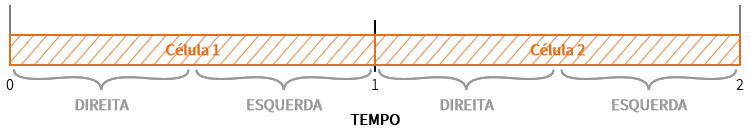
\includegraphics[width=0.87\textwidth]{img/grids_1.png}
\end{center}
\caption{Representação de duas células de uma grelha}
\label{fig:grids-1}
\end{figure}

Na figura \ref{fig:grids-1} podemos ver representadas duas células de uma grelha, cada uma com tamanho de 1 segundo. Também podemos ver que cada célula está dividida em duas partes, direita e esquerda, e a ordem dessas partes pode parecer engano, ou que estão trocadas. Mas estão corretas, pois na verdade cada uma dessas partes é relativa não à célula, mas ao separador das células.

Olhemos por exemplo para o divisor central, situado em cima da marca do 1 segundo. A parte à sua esquerda refere-se à esquerda do separador, e a parte à direita referem-se à direita do separador. Desta forma, faz mais sentido a ordem das partes.

\begin{figure}[h]
\begin{center}
    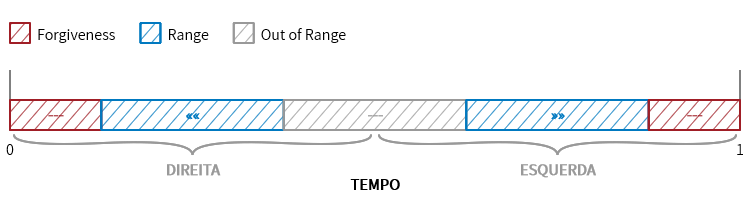
\includegraphics[width=0.87\textwidth]{img/grids_2.png}
\end{center}
\caption{As várias áreas configuráveis de uma grelha}
\label{fig:grids-2}
\end{figure}

Por predefinição, ambas as partes têm o tamanho igual a metade do tamanho da célula (ou seja, neste caso, tanto a parte da esquerda e da direita têm o tamanho de 0.5 segundos). No entanto, é possível customizar o tamanho das duas de forma igual, ou cada uma em particular, através das propriedades \textbf{forgiveness} e \textbf{range}.

\begin{lstlisting}[caption={Código de definição da grelha representada na figura \ref{fig:grids-2}},label={lst:grids-2}]
$grid = Grid( 1,
    forgiveness = 125, # 1/8 of a second
    range = 375        # 3/8 of a second
);
\end{lstlisting}

Não nos esqueçamos que o objetivo da grelha é alinhar eventos, movendo os eventos ao longo do eixo do tempo para junto dos separadores das células. A propriedade \textit{range} tem como valor predefinido metade do tamanho da célula. Isso significa que tanto o \textbf{range\_left} como o \textbf{range\_right} cobrem de modos igual toda a célula, e dessa os eventos são movidos para o separador da grelha que estiver mais próximo. O valor predefinido da propriedade \textit{forgiveness}, por outro lado, é zero, o que significa que mesmo os eventos que se encontrem já muito perto dos separadores são movidos.

Na listagem \ref{lst:grids-2} podemos ver a definição de uma grelha simétrica (as propriedades \textit{left} e \textit{right} são iguais). O valor de \textit{forgiveness} implica que eventos que estejam a mais de 372 milissegundos de distância de qualquer um dos separadores são ignorados pela grelha, isto é, o seu tempo não se mexe. O valor de \textit{forgiveness}, o que significa que eventos que estejam a menos de 125 milissegundos de um dos separadores são também ignorados pela grelha. Neste exemplo, são apenas movidos os eventos que estejam entre 125 e 375 milissegundos de distância de um dos separadores.

Note-se que cada propriedade poderia ser costumizada para a esquerda e para a direita. Isto é, o exemplo a cima podia ser reescrito da seguinte forma:

\begin{lstlisting}[caption={Código alternativo de definição da grelha representada na figura \ref{fig:grids-2}, com as propriedades \textit{left} e \textit{right}},label={lst:grids-3}]
$grid = Grid( 1,
    forgiveness_left = 125,  # 1/8 of a second
    forgiveness_right = 125, # 1/8 of a second
    range_left = 375,        # 3/8 of a second
    range_right = 375        # 3/8 of a second
);
\end{lstlisting}

Se passarmos das propriedades de configuração para a grelha resultante, na verdade cada célula passa a ter dois \textbf{effective ranges}, duas áreas (uma para a esquerda e outra para a direita) onde os eventos que aí calharem são movidos. Os eventos fora dessas áreas são ignorados.

\begin{figure}[h]
\begin{center}
    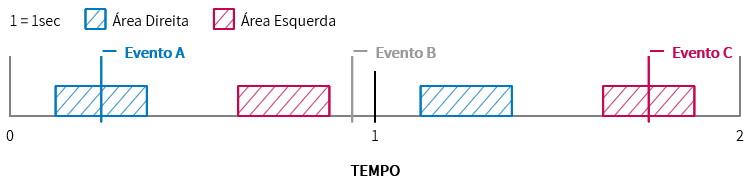
\includegraphics[width=0.75\textwidth]{img/grids_3_1.png}
\end{center}
\vspace*{-5mm}
\caption{Áreas em que a grelha irá mover os eventos, e qual o separador a que pertencem.}
\label{fig:grids-3-1}
\end{figure}

Tomemos como exemplo a seguinte situação com três eventos e a grelha definida anteriormente: o evento A, como calha dentro da área azul (devido à propriedade \textbf{range\_right}), vai ser relocado para o tempo zero. O evento B no entanto, como não calha em nenhuma área (devido devido a propriedade \textbf{forgiveness\_left}. Finalmente, o evento C como calha na área vermelha (devido à propriedade \textbf{range\_left} é relocado para o tempo 2.

\begin{figure}[h]
\begin{center}
    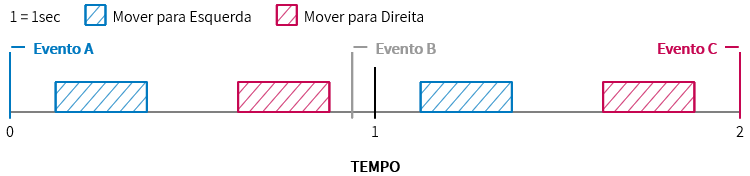
\includegraphics[width=0.85\textwidth]{img/grids_3_2.png}
\end{center}
\vspace*{-5mm}
\caption{Posição dos eventos após o alinhamento com a grelha ter sido aplicado.}
\label{fig:grids-3-2}
\end{figure}

O modo de funcionamento das grelhas pode parecer à primeira vista um desnecessariamente complexo, ou os exemplos um pouco artificiais, mas o objetivo foi sempre permitir ao utilizador aplicar o tipo de grelha que mais se adequar ao seu caso. Isso pode ser uma simples grelha onde só define o tamanho de cada célula, e os \textit{ranges} são cada metade de cada célula, empurrando todos os eventos para o separador que lhe esteja mais próximo, ou exemplos de grelhas assimétricas, onde possivelmente os eventos são sempre movidos só numa direção (esquerda ou direita) ou onde eventos que estejam perto dos separadores não sejam movidos.

\subsection{Teclados Musicais}
Para além de permitir construir expressões que geram sequências de eventos musicais dinâmicas, algo que esteve desde início no topo da nossa lista de prioridades foi sem dúvida adicionar suporte para a criação de teclados interativos. Sendo esta linguagem desenvolvida em computadores, não seria errado pensar que por teclado nos referimos aos teclados físicos dos computadores. E esses fazem certamente parte, mas quando nos referimos a teclados musicais, referi-mo-nos à possibilidade de descrever na nossa linguagem mapeamentos entre \textit{eventos} e expressões musicais ou ações a executar quando esses eventos acontecem.

\begin{lstlisting}[caption={Exemplo de declaração de duas teclas}]
@keyboard {
    a: print( "Tecla a carregada" );
    b: d;
};
\end{lstlisting}

Esses eventos podem então ser teclas de um teclado, mas também de um piano conectado ao computador, ou eventos do rato, ou de qualquer outro dispositivo de \acrshort{io} que as pessoas queiram adaptar, bastando para isso herdar a classe\texttt{KeyboardEvent}.

\subsubsection{Tipos de Eventos}
Os tipos de evento mais comum são teclas de teclado e de piano. Por essa mesma razão implementamos açúcar sintático na definição desses eventos  (que são implementados pelas classes \texttt{KeyStroke} e \texttt{PianoKey}, respetivamente).

\begin{lstlisting}[caption={Declaração de três eventos, o primeiro é uma combinação de teclas, o segundo referência o \textit{virtual key code}, e o terceiro uma nota MIDI}]
@keyboard {
    ctrl+c: ^c;
    [16]: d;
    [c']: e;
};
\end{lstlisting}

A lista de tipos de eventos suportados de base pela linguagem são os seguintes:
\begin{description}
 \item[KeyStroke]
 Este tipo de eventos referem-se às teclas do teclado. Para além de permitirem descrever teclas singulares, também suportam os modificadores \textit{ctrl}, \textit{alt} e \textit{shift}. O evento não carrega consigo nenhum parâmetro extra.
 
 \textbf{Parâmetros:} \textit{N/A}
 \item[PianoKey] Sinalizam quando uma nota é tocada e recebida pela porta MIDI que a aplicação esteja à escuta. Trazem consigo um parâmetro que identifica a velocidade com que a nota foi premida.
 
 \textbf{Parâmetros:} \texttt{\$vel}
 \item[MouseClick] Evento ocorre quando algum dos botões do rato é premido. As informações sobre a posição em que o rato se encontra, bem como qual o botão premido e se foi premido ou levantado, são incluídas como parâmetros deste evento.
 
 \textbf{Parâmetros:} \texttt{\$x}, \texttt{\$y}, \texttt{\$button} \texttt{\$pressed}
 \item[MouseMove] Evento ocorre sempre que o rato é movido. Pode ser útil para controlar alguma variável como se fosse um \textit{slider}. Trás como parâmetros as coordenadas do rato.
 
 \textbf{Parâmetros:} \texttt{\$x}, \texttt{\$y}
 \item[MouseScroll] Evento despoletado quando a roda do rato é acionada. Para além de trazer informações sobre a posição do rato, indica também qual o valor que a roda se moveu, tanto na vertical (mais comum) como também na horizontal.
 
 \textbf{Parâmetros:} \texttt{\$x}, \texttt{\$y}, \texttt{\$dx}, \texttt{\$dy}
\end{description}

Os \textbf{parâmetros} são algo que, como pudemos ver, é disponibilizado por quase todos os tipos de eventos. Eles dão-nos a possibilidade de saber que os eventos foram despoletados, mas saber propriedades sobre o que os despoletou. Estes parâmetros podem ser acedidos passando as variáveis desejadas com o nome do parâmetro (a ordem é irrelevante) à frente da declaração do evento. Essas variáveis podem depois ser acedidas dentro da ação do evento.

\begin{lstlisting}[caption={Teclado que imprime as coordenadas do rato sempre que ele se move}]
@keyboard {
    [keyboard\MouseMove] ($x, $y): print( $x, $y );
};
\end{lstlisting}

Para criar novos tipos de eventos, basta criar uma nova classe em \textit{Python} que derive da classe \texttt{KeyboardEvent}. Esta classe deve implementar apenas dois métodos obrigatórios (\texttt{\_\_hash\_\_} e \texttt{\_\_eq\_\_}) que são usados para guardar os eventos num dicionário, ficando cada evento associado à sua ação. Opcionalmente pode ser definido um terceiro método, \texttt{get\_parameters}, que deve retornar um dicionário com as variáveis e os seus respetivos valores que o evento disponibiliza. Cada tipo de evento pode também definir uma propriedade chamada \texttt{binary} como verdadeira ou falsa.

Os \textbf{binários} referem-se ao conceito de eventos que são conceptualmente compostos por duas fases: premir e soltar. Exemplos deste tipo de eventos são, obviamente premir e soltar teclas do computador ou de um piano. A razão porque este conceito é tratado como um caso particular na nossa linguagem, ao invés de serem tratados como dois eventos separados (\texttt{PianoKeyPress} e \texttt{PianoKeyRelease} por exemplo), deve-se ao facto de os eventos binários mapearem de forma bastante elegante com o conceito de \textit{note on} e \textit{note off} na geração de música. E da mesma maneira que a nossa linguagem não obriga o utilizador a declarar por cada nota o seu ponto de início e de fim separados, não faria sentido fazer isso para os teclados.

Por essa razão, os teclados podem (através dos modificadores \texttt{hold extend} que vamos cobrir a seguir) mapear automaticamente o início e o fim das notas declaradas em cada uma das suas teclas, com os modos \textit{press} e \textit{release} dos seus eventos.

\subsubsection{Modificadores de Eventos}
Cada evento de um teclado tem associada uma ação: essa ação pode ter \textit{size effects}, e opcionalmente retornar um evento musical (ou uma sequência de eventos). Sempre que o evento é despoletado, a ação é avaliada e caso retorne um objeto musical, esse é reproduzido.

Por predefinição, o tempo que a tecla está premida não afeta a duração das notas emitidas. Pelo contrário, a duração das notas (e acordes e todo o resto de eventos musicais) é calculada com o que o utilizador tiver determinado no código. Isto acontece porque o teclado permite que o utilizador defina não só um evento musical para cada tecla, mas sim que possa definir uma música completa, se quiser. Neste caso quando a tecla é premida, a música começa a tocar até terminar.

Os \textbf{modificadores} permitem customizar o comportamento do teclado quando encontra alguma sequência musical. Cada modificador pode ser aplicado a todo o teclado (quando aparece à frente da \textit{keyword} \texttt{@keyboard}), ou ser aplicada individualmente a cada tecla.

\begin{description}
 \item[repeat] Quando presente, o teclado reproduz a música da tecla, e quando esta acabar, começa a tocar novamente, sem parar.
 \item[toggle] Reproduz a música da tecla até esta ser premida novamente (ou a música acabar).
 \item[hold] Reproduz a música da tecla enquanto a tecla estiver premida (ou a música acabar).
 \item[extend] Tanto o \texttt{toggle} como o \texttt{hold} permitem terminar uma música mais cedo. Com este modificador, todas as notas tocadas pela tecla ficam ativas enquanto a pessoa não carregar novamente na tecla (em conjunto com o \texttt{toggle}), ou a largar (em conjunto com o \texttt{hold}).
\end{description}

Assim, se quisermos replicar o comportamento de um piano, por exemplo, em que premir a tecla começa a tocar uma nota, e liberta-la para a nota, podemos usar os modificadores \texttt{hold extend} em conjunto.

\begin{lstlisting}[caption={Aplicar o modificar \texttt{hold extend} a um teclado inteiro}]
@keyboard hold extend {
    a: c;
    s: d:
    d: e;
};
\end{lstlisting}

\subsubsection{Estruturas de Controlo}
Até agora temos visto como é possível declarar manualmente ações num teclado. Algo que ainda não foi dito é o facto de o bloco de declaração de um teclado \verb|@keyboard {}| ser uma macro que, antes da execução, é traduzida para instruções que criam o teclado e registam as teclas.

\begin{lstlisting}[caption={Código gerado automaticamente para criação do teclado descrito no capitulo anterior}]
{
    $__keyboard = keyboard\create();
    keyboard\push_flags($__keyboard; 'hold'; 'extend');
    keyboard\register($__keyboard; 'a'; c);
    keyboard\register($__keyboard; 's'; d);
    keyboard\register($__keyboard; 'd'; e);
    keyboard\pop_flags($__keyboard; 'hold'; 'extend');
    $__keyboard
}
\end{lstlisting}

Vendo desta forma é possível concluir que o código fica extremamente mais verboso, mas ao mesmo tempo abre novas possibilidades: é possível registar teclas condicionalmente, envolvendo a chamada da função num \texttt{if}, ou registar teclas em massa dentro de um ciclo \texttt{for} ou \texttt{while}.

A abordagem de criar os teclados manualmente desta forma é sem dúvida válida para os casos mais complexos (com alguns dos teclados definidos na biblioteca \textit{standard} a serem criados desta forma). Mas achamos que seria interessante poder integrar este tipo de estruturas de controlo simples com a sintaxe específica de declaração de teclados, para permitir mais variedade ao tipo de teclados que são possíveis de criar com ela.

Assim sendo, dentro da expressão de declaração de teclados, são suportados os seguintes construtores sintáticos:
\begin{description}
 \item[Condicionais] Permitem tornar a declaração de uma ou mais teclas condicionais. O código gerado é transformado de forma a envolver as funções que registam as teclas dentro de um \texttt{if}.
 \item[Ciclos] É possível ter também ciclos \texttt{for} e \texttt{while} dentro de um teclado. Isto permite percorrer um \textit{array} ou repetir a mesma tecla com alguma variação várias vezes.
 \item[Blocos] É possível envolver instruções da linguagem em chavetas em qualquer parte dos teclados.
\end{description}

Tomemos um pequeno exemplo que associa a quatro teclas a ação de imprimir para o ecrã um número. Podemos ver que é possível encadear os construtores uns dentro dos outros (neste caso um \texttt{if} dentro de um \texttt{for}). Mas mais interessante do que isso, é verificarmos que existe um pequeno bloco de código responsável por declarar a variável \texttt{\$ki = \$i}, e que no \texttt{print} são impressos as duas variáveis.

\begin{lstlisting}[caption={Declaração de teclado dinâmica recorrendo ao uso de ciclos, condicionais e blocos de código.}]
$i = 0;

@keyboard {
    for ($k in @[ 'a', 's', 'd', 'f' ]) {
        if ($i > 0) {
            { $ki = $i };
            [$k] hold extend: print( $i, $ki );
        };
        { $i += 1 };
    }
};
\end{lstlisting}

Não seria invulgar pensar que ambos os números seriam iguais sempre que fossem impressos, mas isso não é o caso. Isto providencia uma boa ocasião para reforçar a noção que as teclas ficam associadas a expressões, e essas expressões são executadas só quando a tecla é ativada.

Isto significa que quando qualquer tecla for premida, o valor de \texttt{\$i} será sempre o mesmo: $4$. Isto porque a variável está declarada fora do teclado, e mais importante, fora do ciclo \texttt{for}, o que significa que todas as teclas referenciam a mesma variável. Por outro lado, a variável \texttt{\$ki} é declarada pela primeira vez dentro do ciclo, e como tal está a criar quatro símbolos diferentes que são depois cada um referenciado pela tecla respetiva.

\subsubsection{Gravar e Reproduzir Performances}
Uma vez criado um ou mais teclados, o som produzidos por eles é direcionado automaticamente para os \textit{outputs} (por predefinição as colunas de som). No entanto, é possível instruir os teclados para guardarem num ficheiro de \textit{performance} uma lista das teclas ativadas. Isto permite depois ao utilizador reproduzir uma performance gravada, ou até efetuar modificações a essa gravação.

\begin{lstlisting}[caption={Gravação de uma \textit{performance}},label={lst:kb-perf-1}]
keyboard\record( $file );
\end{lstlisting}

Através da função descrita na listagem \ref{lst:kb-perf-1}, é possível instruir os teclados para gravarem para um determinado ficheiro, cujo caminho é passado como argumento. Também é possível passar o valor \texttt{none} para a função, o que efetivamente termina a gravação da performance atual (se estiver a decorrer alguma).
De notar que uma vez que os teclados suportam registar como ações, não só expressões musicais, mas também quaisquer blocos de códigos válidos, podemos chamar esta função na ação de uma das teclas do teclado. Desta forma é possível iniciar e parar a gravação durante a execução do programa.

\begin{lstlisting}[caption={Reprodução de uma \textit{performance}},label={lst:kb-perf-2}]
keyboard\replay( $file, $delay = 0 );
\end{lstlisting}

Da mesma maneira que é possível gravar uma \textit{performance}, é possível também reproduzir uma \textit{performance} a qualquer momento através da função referenciada em \ref{lst:kb-perf-2}. Neste caso devemos passar o caminho do ficheiro contendo a \textit{performance} gravada, bem como um parâmetro opcional (em milissegundos) para atrasar o início da reprodução durante algum tempo. Isto pode ser útil se quisermos tocar alguma faixa ao vivo por cima da gravação, para alinhar a mesma ou para servir de tempo de preparação.

\begin{lstlisting}[caption={Conversão de uma \textit{performance} numa sequência de eventos músicais},label={lst:kb-perf-3}]
$music = keyboard\readperf( $file, $keyboards = [] );
\end{lstlisting}

Mas podemos não querer reproduzir diretamente uma \textit{performance}. Também é possível carregar uma \textit{performance} gravada para memória, como uma sequência de eventos musicais convencional, que podemos depois manipular com todas as funções e operadores que já vimos e que operam sobre música.

Esta função aceita também, para além do usual caminho do ficheiro de \textit{performance}, uma lista opcional de teclados a usar na conversão. Quando a lista vai vazia, são utilizados todos os teclados ativos. Isto demonstra uma das funcionalidades mais interessantes da gravação de ficheiros de \textit{performance}, na medida que permitem gravar os eventos das teclas ativadas, mas podemos depois reproduzir essas \textit{performances} com teclados com notas e expressões diferentes associadas às teclas.



\subsubsection{Buffers}
Ao contrário de \textit{performances}, que gravam os eventos que acionam as teclas dos teclados, é possível guardar diretamente os eventos musicais produzidos pelos teclados com a \textit{class} \texttt{keyboard\textbackslash{}Buffer}. Os eventos capturados em \textit{buffers} podem ser tratados como qualquer outra sequência musical, e como tal, ser composta com outras expressões, passada a funções e tudo o resto que a linguagem possibilita. 

\begin{lstlisting}[caption={Instanciação de um \textit{buffer}}]
$buffer = keyboard\Buffer( $keyboards = ..., $start = true );
\end{lstlisting}
Ao construir um \textit{buffer}, por predefinição, todos os teclados são gravados imediatamente. É no entanto possível passar uma lista a limitar quais os teclados que irão ser gravados para o \textit{buffer}, útil para permitir dividir as notas gravadas em faixas separadas (um \textit{buffer} grava uma faixa, outro grava uma faixa diferente, etc). Para além disso, é possível também não iniciar a gravação para o \textit{buffer} imediatamente. 

Entre as funcionalidades disponibilizadas pela classe, podemos destacar as mais importantes como sendo:
\begin{description}
 \item[start] Começa a gravar os eventos emitidos. Mesmo depois de chamado o método \texttt{start()}, o \textit{buffer} só inicia a gravação quando for capturado o primeiro evento musical. Caso se queira forçar um \textit{padding} silencioso ao início, pode-se emitir um evento de pausa com duração zero. Caso o \textit{buffer} já tenha conteúdos em memória, o que for gravado agora é acrescentado ao fim.
 \item[stop] Para a gravação do \textit{buffer}. Mais uma vez, a gravação é cortada no último evento musical. Caso se queira forçar a duração do \textit{buffer} com mais algum tempo depois da última nota, basta emitir um evento de pausa com duração zero quando realmente quisermos que o \textit{buffer} termine.
 \item[clear] Limpa tudo o que o \textit{buffer} tiver gravado e permite reutilizar o \textit{buffer} do inicio.
 \item[to\_music] Retorna os conteúdos do \textit{buffer} na forma de uma sequência musical. Esta sequência é imutável: alterações aos conteúdos do \textit{buffer} não são refletidos nos dados da sequência gerada. Para obter essas alterações, este método deve ser chamado novamente, retornando uma nova sequência musical.
 \item[from\_music] Permite substituir manualmente o conteúdo do \textit{buffer} com uma sequência musical. É útil como iremos ver mais à frente para permitir as operações de \texttt{save()} e \texttt{load()} dos \textit{buffers}.
\end{description}

Tudo isto permite manipular os \textit{buffers} através da linguagem de \textit{scripting}, mas sendo o objetivo dos \textit{buffers} serem usados em conjunto com os teclados, primariamente quando o utilizador os estiver a usar para compor arranjos musicais, é desejável associar todas estas chamadas de código a teclas do teclado, para as permitir usar durante a sua utilização.

Tendo acesso às funções dos \textit{buffers}, cada utilizador pode então programar a sua utilização como bem quiser. Mas para os casos mais comuns, a biblioteca da linguagem fornece já funções destinadas a facilitar o seu uso.

\begin{lstlisting}[caption={Funções disponibilizadas para criação de \textit{buffers} controlados por teclados.}]
keyboard\bufslot( $bf = keyboard\Buffer( start = false ), $key = "p" );

keyboard\bufpad( ref $buffers, $keys = @[ '0', '1', '2', '3', '4', '5', '6', '7', '8', '9' ], $savename = "buffers.mkl", $load_key = 'f7', $save_key = 'f8' );
\end{lstlisting}

A primeira função \texttt{keyboard\textbackslash{}bufslot} permite criar apenas um \textit{buffer} associado a uma tecla.

A segunda \texttt{keyboard\textbackslash{}bufpad} função permite uma utilização mais avançada, associando $N$ \textit{buffers} distintos a $N$ teclas. Para além de permitir iniciar e parar de gravar, bem como reproduzir os conteúdos de cada \textit{buffer}, também permitem gravar e carregar os conteúdos dos \textit{buffers}.

Quando o utilizador pressiona a tecla para gravar ou carregar os \textit{buffers}, é mostrado ao utilizador uma \textit{dialog} para escolher o caminho onde guardar. O caminho introduzido pelo utilizador fica guardado em memória e é preenchido automaticamente da próxima vez que a \textit{dialog} for mostrada, evitando obrigar o utilizador a escrever o caminho de todas as vezes.

\begin{figure}[h]
\begin{center}
    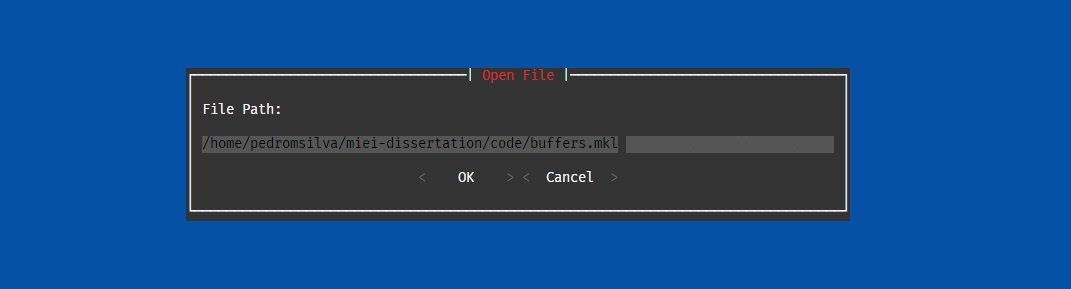
\includegraphics[width=0.87\textwidth]{img/open_buffers_dialog.png}
\end{center}
\caption{Janela de carregamento dos \textit{buffers}}
\end{figure}

Os conteúdos do \textit{buffer} são guardados num ficheiro \texttt{.mkl}, o que é bastante interessante pois permite evitar ter de criar e implementar algum formato específico para guardar os seus conteúdos. Mas também permite, sendo um formato de texto, e sendo a sua sintaxe a da nossa linguagem \textit{Musikla}, o utilizador pode gravar os \textit{buffers}, abrir o ficheiro com algum editor de texto e efetuar alterações manualmente, e carregar essas alterações de novo para os \textit{buffers} com extrema facilidade.

\begin{lstlisting}[caption={Formato do ficheiro de gravação dos \textit{buffers}.}]
$buffers = @{};
$buffers::set(1; (:default r2/23 [B^d^f]1/29 r1/32 [A^ce]1/32))
\end{lstlisting}

O formato do ficheiro passa pela declaração de uma variável \textbf{\$buffers} contendo um dicionário. O dicionário contém depois um par chave-valor para cada \textit{buffer} não vazio aquando da gravação do ficheiro. A chave representa o índice do \textit{buffer}, e o valor representa a sequência musical lá guardada nesse momento.

Para guardar o ficheiro, é criada é memória a sua \acrshort{ast} respetiva. Esta é depois convertida em texto através da classe \texttt{CodePrinter}.

O processo de carregar o ficheiro é igualmente simples, passando por executar o \textit{script} num contexto isolado. Depois o valor da variável \texttt{\$buffers} é obtido, e as entradas do dicionário são percorridas, substituindo os valores presentes nos \textit{buffers} recorrendo à função \texttt{keyboard\textbackslash{}Buffer.from\_music()}.

\subsection{Editor Embutido}
O modo principal de execução de código baseia-se em carregar um ficheiro \textit{Musikla} e executá-lo. Mas ao mesmo tempo, uma das funcionalidades mais importantes da linguagem é permitir descrever teclados musicais que permitem interação do utilizador enquanto a aplicação não for fechada.

No entanto, muitas das funcionalidades disponibilizadas pela aplicação são acessíveis através de classes e funções que podem ser chamadas pela linguagem. Isto tipicamente envolve uma de duas opções: o utilizador ter de mudar o ficheiro de código e executá-lo novamente, o que implica perder os dados que estejam em memória (como \textit{buffers} e o possível estado do teclado). Também é possível associar pedaços de código a ações do teclado para permitir chamar esses pedaços de código durante a execução do programa, mas isso implica ser necessário planear todos os possíveis casos de uso à partida antes de iniciar executar o teclado. Se nos esquecermos de alguma, temos de voltar à opção inicial de mudar o código fonte e reiniciar a aplicação.

A solução passa pela inclusão de um simples editor de texto em \textit{runtime} (implementado com recurso ao módulo \textit{Python} \texttt{prompt\_toolkit}. A biblioteca dispõem de uma função para permitir abrir e fechar o editor de texto ao premir uma tecla, ou também uma função para abrir diretamente o editor quando é chamada, dando assim ao utilizador mais controlo sobre como é possível usar este editor.

\begin{lstlisting}[caption={Abre o editor quando a tecla \textbackslash{} é premida},label={lst:kb-editor-1}]
keyboard\repl( $key = "\\", $ctx = none );
\end{lstlisting}

Na listagem \ref{lst:kb-editor-1} é possível ver a função que permite abrir o editor embutido. É também possível passar um contexto através do qual as expressões do editor irão ser avaliadas. Isto pode afetar quais as variáveis que são visíveis, ou até ter vários editores para diferentes contextos.

\begin{figure}[h]
\begin{center}
    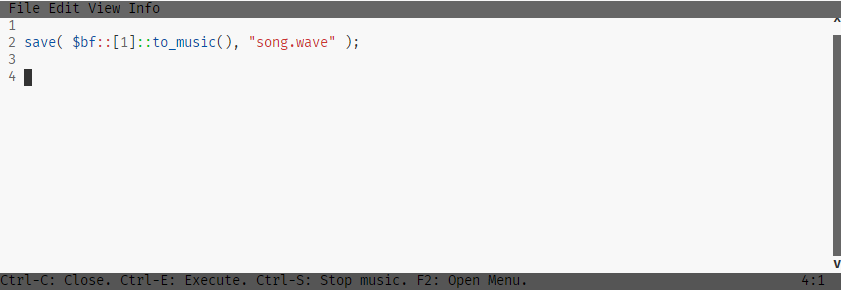
\includegraphics[width=0.87\textwidth]{img/embedded_editor.png}
\end{center}
\caption{Interface do editor embutido.}
\end{figure}

\begin{lstlisting}[caption={Abrir manualmente o editor},label={lst:kb-editor-2}]
keyboard\open_repl( $cb = none );
\end{lstlisting}

Se não quisermos que o editor seja aberto simplesmente quando uma tecla é carregada, podemos chamar manualmente a função para o abrir. Isto tem a vantagem de podermos passar um \textit{callback} ao editor para sermos notificados quando o editor é fechado. 
Isto significa que o editor pode ser usado não só como um ambiente de programação \textit{Musikla} genérico, mas também como um modo de \textit{input} de texto genérico a ser usado pelo utilizador.

\begin{figure}[h]
\begin{center}
    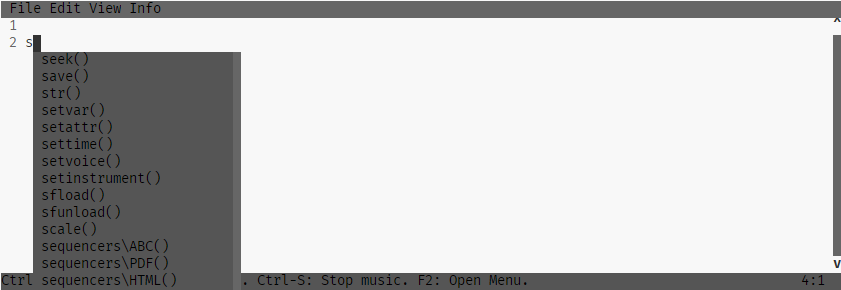
\includegraphics[width=0.87\textwidth]{img/embedded_editor_autocomplete.png}
\end{center}
\caption{Implementação básica de uma solução de \textit{auto-complete}.}
\end{figure}

Como prova de conceito, também foi incorporado um sistema de \textit{auto-complete} que sugere símbolos que estejam declarados no nível base do contexto. Devido ao facto de o editor estar a correr ao mesmo tempo que a aplicação, esta funcionalidade não foi implementada através da análise dos ficheiros de código. Em vez disso, o objeto de contexto é analisado em tempo real para listar quais os símbolos que estão acessíveis.

Esta funcionalidade é extremamente útil tendo em conta que a linguagem tem como público alvo músicos que podem não ser programadores experientes. Por isso mesmo, ter um ambiente que assista o utilizador a saber quais as variáveis e métodos que pode utilizar.

No futuro, era interessante melhorar o \textit{auto-complete} para completar sub-propriedades de objetos e listas, bem como mostrar informações adicionais sobre as sugestões, tal como os seus tipos e no caso de serem métodos, quais os parâmetros que aceita.

\subsection{Transformadores}
Os transformadores são uma solução para um problema prático que surgiu durante o desenvolvimento do projeto, ao invés de serem uma funcionalidade pública da linguagem. No entanto a razão pela qual foram necessários, bem como a solução desenvolvida, podem ser interessantes de serem discutidas. Para compreendermos melhor a razão da sua necessidade, imaginemos o seguinte caso.

\subsubsection{O Problema}

Um dos tipos de dados mais importantes na nossa linguagem é o tipo música, que como já referimos várias vezes pode ser representado como uma sequência de eventos musicais. Quando pensamos em sequências, é fácil imaginar uma variedade de operações genéricas possíveis de serem aplicadas nelas, como \texttt{map} e \texttt{filter}. 

Mas também existem operações mais específicas ao nosso caso que podemos querer aplicar, como dada uma sequência de eventos, separar os \texttt{NoteEvent} em dois \texttt{NoteOnEvent} e \texttt{NoteOffEvent}. Isto à primeira vista pode parecer um simples \texttt{flatMap}, em que alguns eventos são transformados em dois a serem inseridos na sequência. No entanto, uma vez que os eventos nas nossas sequências devem viajar sempre ordenados, não podemos simplesmente inserir o evento \textit{off} junto do \textit{on}, porque podem existir outros eventos que comecem ao mesmo tempo ou depois da nossa nota começar, mas antes dela acabar.

Nesse caso basta construirmos uma algoritmo simples que guarde num \textit{buffer} ordenado os eventos \textit{off}, e os vá inserido imediatamente atrás do primeiro evento com um \textit{timestamp} maior que os seus.

E como este, existem vários algoritmos que podem ser usados e reutilizados em diversas partes da aplicação com os mais diversos propósitos de transformar sequências de eventos.

O problema surge quando a fonte da música pode ser sincrona (no caso de uma expressão da nossa linguagem) ou assíncrona (no caso de um teclado ou piano, em que os eventos vão sendo gerados em tempo real). \textit{Python} suporta assincronia através do módulo \texttt{asyncio} que pode ser usado em conjunto com a sintaxe \textit{async/await}.

Para simplificar os exemplos seguintes, tomemos o caso da operação genérica \textit{map}. As suas implementações, nas variantes síncrona e assíncrona, poderiam ser descritas como visto na listagem \ref{lst:transformers-map}.

\begin{lstlisting}[caption={Exemplo de uma função \texttt{map} com versões sincronas e asíncronas},label={lst:transformers-map},language=Python]
def map (fn):
    for event in music:
        yield fn(event)

async def map_async (fn):
    async for event in music:
        yield fn(event)
\end{lstlisting}

Como podemos ver, quando a única diferença no algoritmo é se a \textbf{fonte é síncrona ou assíncrona}, a variação é mínima. Mas a diferença é sintática, por isso teríamos duas escolhas:
\begin{itemize}
 \item Para cada algoritmo criar duas versões, uma síncrona e outra assíncrona. Mas isto levava a duplicação de código particularmente má, porque o que iria mudar eram apenas \textbf{duas palavras} em todas as funções.
 
 \item Usar sempre a versão assíncrona, mesmo quando a fonte dos dados é síncrona. Isto porque é sempre possível converter uma sequência de dados síncrona em assíncrona, mas o inverso já não é. O problema desta solução é o facto de as funções assíncronas terem \textit{cor}\footnote{\url{https://journal.stuffwithstuff.com/2015/02/01/what-color-is-your-function/}}, e só poderem ser chamadas por funções da mesma cor. Qualquer função que potencialmente lidasse com expressões musicais teria de passar a ser assíncrona. E como a nossa linguagem tem tipos dinâmicos, potencialmente qualquer expressão pode retornar uma sequência musical, logo \textbf{todas as expressões} na nossa linguagem teriam de ser executadas em modo assíncrono, o que traria uma penalização a nível de \textit{performance} difícil de justificar.
\end{itemize}


\subsubsection{A Solução Escolhida}
A solução passou por criar uma abstração a que chamamos \textbf{Transformador}, que contém um bocado das duas opções anteriores: Os algoritmos são declarados apenas uma vez, e são depois envoltos num \textit{transformador} que disponibiliza duas interfaces públicas, uma síncrona e outra assíncrona. Cada transformador tem uma interface pública composta por 4 funções que permitem simular um iterador: \verb|add_input( ev )|, \verb|end_input()|, \verb|add_output( ev )| e \verb|end_output()|.

Para evitar chamar manualmente as funções e tratar do controlo do fluxo de execução manualmente, são incluídos dois métodos de classe em todos os transformadores que permitem correr um iterador (síncrono ou assíncrono). As funções, chamadas \texttt{iter} e \texttt{aiter} recebem (e retornam) respetivamente um iterador síncrono e assíncrono.

Vejamos agora um exemplo do transformador \textbf{map} na listagem \ref{lst:transformers-map}. Pode parecer bastante mais verbosa do que as funções \textit{map} iniciais, mas é importante notar que este custo é fixo: só esta parte do algoritmo muda, e todo o resto seria igual. Como os transformadores utilizados no projeto são bem mais complexos do que este pequeno exemplo (podendo ter mais de uma centena de linhas de código), este custo fixo de escrever cerca de seis linhas de código \textit{boilerplate} por transformador não é um problema tão grande.

\begin{lstlisting}[caption={Implementação da função \texttt{map} usando a nossa abordagem de transformadores},label={lst:transformers-map},language=Python]
class MapTransformer(Transformer):
    def __init__ (self, fn):
        self.fn = fn
    
    def transform ( self ):
        while True:
            done, value = yield

            if done: break
            
            self.add_output( self.fn( value ) )
\end{lstlisting}

Todos os transformadores implementam uma função gerador \textit{transform}, que é a peça central de tudo isto. Aí dentro, temos um ciclo responsável por emular a iteração sobre a sequência de \textit{input}. Depois utilizamos a instrução \textit{yield} para obter o próximo valor. Aqui estamos a aproveitar o facto de esta instrução não permitir apenas enviar valores para fora do gerador (que é o seu uso mais comum), mas também receber valores. Desta forma o gerador fica em pausa até receber o próximo evento. A vantagem desta pausa é que pode ser retomada logo de seguida se estivermos a trabalhar com iteradores síncronos, ou pode ficar assim até o próximo valor ficar disponível, no caso de um iterador assíncrono.

\begin{lstlisting}[caption={Exemplo de um transformador \texttt{map} e da sua utilização},label={lst:transformers-map-usage},language=Python]
# Irá imprimir 0, 2, 4, 6, 8
for ev in MapTransformer.iter( range( 5 ), lambda e: e * 2 ):
    print( ev )
\end{lstlisting}

Na listagem \ref{lst:transformers-map-usage} podemos ver a utilização do transformador aplicada a uma lista (já que também implementam a interface de um iterador). O método \texttt{aiter} poderia ser usado de forma análoga com um \textit{async for} e com um iterador assíncrono.


\section{Resumo do Desenvolvimento}
O processo de desenvolvimento foi bastante ágil, sendo estruturado de uma forma iterativa, em que a cada semana eram implementadas novas funcionalidades. Estas podiam depois ser postas à prova, aplicadas a casos de estudo, e possivelmente melhoradas numa iteração futura.

O tempo dedicado a cada um dos componentes da linguagem Musikla foi intercalado entre a análise sintática, semântica dinâmica e a biblioteca \textit{standard}. Nem todas as funcionalidades exigiram esforço ou tempo equivalentes, e apesar de linhas de código não mapearem perfeitamente para tempo despendido, permitem ter alguma noção aproximada do mesmo.

\begin{table}[h]
\centering
\def\arraystretch{1.3}
\begin{tabular}{lcc}
\rowcolor[HTML]{EFEFEF} 
\textbf{Componente}          & \multicolumn{1}{l}{\cellcolor[HTML]{EFEFEF}\textbf{Linhas de Código}} & \multicolumn{1}{l}{\cellcolor[HTML]{EFEFEF}\textbf{Percentagem}} \\
\textbf{Análise Sintática}   & 1090                                                                  & 11\%                                                             \\
\textbf{Semântica Dinâmica}  & 5268                                                                  & 53\%                                                             \\
\textbf{Biblioteca Standard} & 3527                                                                  & 36\%                                                             \\ \hline
\textbf{Total}               & 9885                                                                  & 100\%                                                           
\end{tabular}
\caption{Linhas de código (sem linhas vazias ou de comentário) do projeto Musikla}
\label{tab:loc}
\end{table}

Obviamente sendo estes números apenas uma contagem das linhas atuais, não são uma representação total de tudo o que foi programado, pois não têm em conta partes do código que foram  reescritas ao longo do desenvolvimento, como foi o caso da gramática e do reconhecedor sintático, por exemplo.

Para além destes componentes, foi desenvolvido para ser usado na documentação um utilitário em \textit{JavaScript}\footnote{Código disponível em \url{https://github.com/pedromsilvapt/miei-dissertation/blob/master/code/musikla/docs/assets/generator.js}} com cerca de 500 linhas de código, que permite descrever e gerar os diagramas sobre grelhas (também usados nesta dissertação). A documentação está escrita no formato \textit{Markdown} e conta também com um pouco mais de 700 linhas de texto. Este número não pode no entanto ser comparado diretamente com as linhas de código, já que texto em prosa e código são conceitos diferentes. Ainda assim ajudam a ter ideia do que foi feito, para além da escrita da desta dissertação, do artigo publicado e do desenvolvimento do interpretador Musikla.

\chapter{Guia Rápido de Utilização}
O resultado final do processo de desenho e desenvolvimento descrito a cima foi um módulo \textit{Python} publicado no repositório \textit{PyPi} chamado \texttt{musikla}. Este módulo pode ser usado através da linha de comandos, ou os seus sub-módulos podem ser usados diretamente num projeto \textit{Python}.

Nesta secção vamos fazer uma pequena \textit{overview} dos diversos modos de como o módulo pode ser utilizado (versão da documentação mais completa disponível em na \href{https://pedromsilvapt.github.io/miei-dissertation/}{web}).

A instalação é bastante simples, sendo suficiente correr o comando seguinte comando:

\begin{lstlisting}[caption={Processo de instalação do \textit{package} musikla},label={lst:install-musikla},language=Bash]
pip install musikla
\end{lstlisting}

É importante notar que uma dependência central da linguagem é a biblioteca nativa \textit{FluidSynth}. Apesar de existir uma versão \texttt{2.x}, essa não é suportada, pelo que é necessário o utilizador certificar-se que o seu sistema tem a versão \texttt{1.x} instalada.

\section{Módulos}
O projeto \textbf{musikla} está dividido em bastantes sub-módulos, os mais importantes dos quais são listados aqui:

\begin{description}
 \item[musikla.core.theory] Contém classes e funções auxiliares relativas à teoria músical, utilizadas por diversos outros sub-módulos.
 \item[musikla.core.events.transformers] Alberga os transformadores responsáveis por separar notas musicais em eventos On/Off, por exemplo, ou por tentar agrupar notas concorrentes em acordes, se for o caso disso, entre muitos mais.
 \item[musikla.core.events] Contém as classes que representam os eventos musicais em memória, desde os mais óbvios, como o \texttt{NoteEvent}, \texttt{ChordEvent} ou \texttt{RestEvent}, mas também outros menos óbvios como o \texttt{ControlChangeEvent}, por exemplo.
 \item[musikla.core] Disponibiliza muitas das classes mais fundamentais para o funcionamento da linguagem, tais como \texttt{Context}, \texttt{Music}, \texttt{Instrument}, \texttt{Voice}, \texttt{SymbolsScope}, entre outros.
 \item[musikla.parser.abstract\_syntax\_tree] Contém as classes que representam os diversos nós da \acrshort{ast}.
 \item[musikla.parser] Disponibiliza as classes \texttt{Parser}, responsáveis por criar uma \acrshort{ast} com base numa \textit{string} ou num ficheiro contendo código Musikla, bem como a classe \texttt{CodePrinter} responsável pelo processo oposto, transformando de volta uma \acrshort{ast} numa \textit{string} usando a sintaxe da linguagem.
 \item[musikla.audio.sequencers] Alberga os diversos sequênciadores (formatos de saída) suportados nativamente pela linguagem.
 \item[musikla.audio] Contém as classes \texttt{Player} e \texttt{InteractivePlayer} que permitem reproduzir sequências musicais para os sequenciadores.
 \item[musikla.libraries] Disponibilizam as várias classes que definem as funções e símbolos expostos para a linguagem Musikla pela biblioteca \textit{standard}.
 \item[musikla] O módulo  principal, contém as duas classes responsáveis por inicializar todos os sistemas necessários para a linguagem funcionar, \texttt{CliApplication} e \texttt{Script}.
\end{description}

\section{Configuração}
Quando a aplicação é inicializada, é opcionalmente carregado um ficheiro \texttt{musikla.ini} se este se encontrar na pasta \textit{Home} do computador do utilizador. Este ficheiro permite configurar diversos dos valores por predefinição utilizados pela linguagem. A maioria destas propriedades pode ser substituída e costumizada em cada execução quando a linguagem é executada pelo terminal.

\begin{lstlisting}[caption={Exemplo de um ficheiro de configuração da linguagem},label={lst:configuration-file}]
[Musikla]
soundfont = /path/to/soundfont.sf2
output = -o alsa
midi_input = midi input port name
path = colon : separated list of paths to search for when importing files
prelude = colon : separated list of paths to include in the prelude (what is available to all modules)
autoload = colon : separated list of paths to execute before the main file does

[FluidSynth.Settings]
audio.periods = 2
audio.period-size = 64
synth.sample-rate = 44100
\end{lstlisting}

O valor da propriedade \textbf{soundfont} indica o caminho do ficheiro \texttt{.sf2} a usar pela linguagem para sintetizar os sons.

A propriedade \textbf{output} permite indicar qual ou quais os sequênciadores (e os seus parâmetros) a serem por predefinição utilizados quando o utilizador não especifica nenhum em particular. A sua sintaxe é explicada em mais detalhe no capítulo seguinte.

A propriedade \textbf{midi\_input} permite indicar o nome da porta \textit{MIDI} a usar quando algum teclado está à escuta de eventos \textit{MIDI}.

A propriedade \textbf{path} permite listar um conjunto de caminhos que serão procurados sempre que o utilizador importe algum ficheiro global nos seus \textit{scripts}.

A propriedade \textbf{prelude} indica uma lista de \textit{scripts} Musikla a serem executados e carregados, e cujos símbolos exportados devem ficar disponíveis para todos os outros módulos.

A propriedade \textbf{autoload} é similar à \texttt{prelude}, mas os símbolos apenas são disponibilizados para o ficheiro que o utilizador estiver a correr diretamente (o ficheiro \textit{entry point}, podemos dizer).

Na secção \textbf{FluidSynth.Settings} podemos alterar manualmente as propriedades passadas ao sequênciador \textit{FluidSynth}. A lista de propriedades e valores suportados está disponível \href{http://www.fluidsynth.org/api/fluidsettings.xml}{aqui}\footnote{FluidSettings.xml \url{http://www.fluidsynth.org/api/fluidsettings.xml}}.


\section{Linha de Comandos}
A linha de comandos pode ser executada através do comando \texttt{musikla}. Podemos executar um ficheiro passando o seu caminho como argumento. Também podemos correr \texttt{musikla --help} para vermos uma listagem dos argumentos suportados.

\begin{lstlisting}[caption={Exemplo de um ficheiro de configuração da linguagem},label={lst:configuration-file},language=Bash]
musikla file.mkl --soundfont custom_soundfont.sf2
    -o alsa --gain 1
    -o music.wav
    -o musikla_port -f midi --port
\end{lstlisting}

O comando pode ter uma lista de seuquênciadores (ou \textit{outputs}) para utilizar. Estes devem vir sempre no fim do comando, depois de todos os argumentos e opções globais, e são identificados pela opção \texttt{-o} ou \texttt{--output}. O tipo do sequênciador é geralmente inferido pelo valor passado ao output, mas caso haja ambiguidade, é possível identificar manualmente o formato com a opção \texttt{-f} ou \texttt{--format}. Também são passadas a esse \textit{output} todas as opções que estiverem depois do \texttt{-o} e até ao fim do comando, ou até ao próximo \texttt{-o} encontrado. As opções aceites variam com o formato do \textit{output}.

